% 本册使用用户提供的 ElegantBook 4.7 原版文类，文类文件保持不变。
% 模板许可 LPPL 1.3c+，详见 licenses/ElegantBook-License.txt。
% XeLaTeX 编译两遍。正文与原示范教案同源，仅重排层级与动态交叉引用。
\documentclass[lang=cn,11pt,oneside,openany,chinesefont=nofont,color=blue,titlestyle=hang]{elegantbook}
\setCJKmainfont{FandolSong-Regular.otf}[BoldFont=FandolSong-Bold.otf,ItalicFont=FandolKai-Regular.otf]
\setCJKsansfont{FandolHei-Regular.otf}[BoldFont=FandolHei-Bold.otf]
\setCJKmonofont{FandolFang-Regular.otf}
\setCJKfamilyfont{zhsong}{FandolSong-Regular.otf}[BoldFont=FandolSong-Bold.otf]
\setCJKfamilyfont{zhhei}{FandolHei-Regular.otf}[BoldFont=FandolHei-Bold.otf]
\setCJKfamilyfont{zhkai}{FandolKai-Regular.otf}
\setCJKfamilyfont{zhfs}{FandolFang-Regular.otf}
\providecommand{\heiti}{\CJKfamily{zhhei}}\providecommand{\songti}{\CJKfamily{zhsong}}\providecommand{\kaishu}{\CJKfamily{zhkai}}\providecommand{\fangsong}{\CJKfamily{zhfs}}
\usepackage{longtable,tabularx,array,caption,needspace,lastpage,xurl}
\graphicspath{{assets/}}
\definecolor{Navy}{HTML}{173754}
\definecolor{Teal}{HTML}{2C8586}
\definecolor{Gold}{HTML}{BA9657}
\definecolor{Pale}{HTML}{F1F5F7}
\definecolor{Line}{HTML}{D8E1E6}
\definecolor{Muted}{HTML}{6B7F8A}

% 整册统一底色与几何页边纹理，所有页（包括封面、目录、正文和附件）共用。
\definecolor{Paper}{HTML}{F5F8F7}
\definecolor{PaleTeal}{HTML}{E5EFEE}
\definecolor{PaleGold}{HTML}{EEE8DB}
\AddToHook{shipout/background}{%
\begin{tikzpicture}[remember picture,overlay]
\fill[Paper] (current page.south west) rectangle (current page.north east);
\fill[PaleTeal] (current page.north east)--([xshift=-4.2cm]current page.north east)--([yshift=-2.25cm]current page.north east)--cycle;
\fill[PaleTeal] (current page.south west)--([xshift=3.5cm]current page.south west)--([yshift=1.9cm]current page.south west)--cycle;
\fill[Teal!14!Paper] (current page.north west) rectangle ([xshift=.22cm]current page.south west);
\fill[Navy] (current page.south west) rectangle ([yshift=.18cm]current page.south east);
\fill[Gold] ([xshift=12.6cm,yshift=.18cm]current page.south west)--([xshift=15.1cm,yshift=.18cm]current page.south west)--([xshift=15.65cm,yshift=.40cm]current page.south west)--([xshift=13.15cm,yshift=.40cm]current page.south west)--cycle;
\end{tikzpicture}}
% GitHub Pages公开网页的实际链接。
\newcommand{\PublicBaseURL}{https://profwangqi.github.io/\%E8\%AF\%BE\%E4\%BB\%B6/\%E6\%9C\%AC\%E7\%A7\%91\%E6\%95\%99\%E5\%AD\%A6/\%E5\%9B\%BD\%E9\%99\%85\%E9\%87\%91\%E8\%9E\%8D/\%E7\%A4\%BA\%E8\%8C\%83\%E6\%95\%99\%E5\%AD\%A6/}
\newcommand{\CourseEntryURL}{https://profwangqi.github.io/\%E8\%AF\%BE\%E4\%BB\%B6/\%E6\%9C\%AC\%E7\%A7\%91\%E6\%95\%99\%E5\%AD\%A6/\%E5\%9B\%BD\%E9\%99\%85\%E9\%87\%91\%E8\%9E\%8D/\%E7\%A4\%BA\%E8\%8C\%83\%E6\%95\%99\%E5\%AD\%A6/\#top}
\newcommand{\RiskLabURL}{https://profwangqi.github.io/\%E8\%AF\%BE\%E4\%BB\%B6/\%E6\%9C\%AC\%E7\%A7\%91\%E6\%95\%99\%E5\%AD\%A6/\%E5\%9B\%BD\%E9\%99\%85\%E9\%87\%91\%E8\%9E\%8D/\%E7\%A4\%BA\%E8\%8C\%83\%E6\%95\%99\%E5\%AD\%A6/\#risk-lab}
\newcommand{\AIReviewURL}{https://profwangqi.github.io/\%E8\%AF\%BE\%E4\%BB\%B6/\%E6\%9C\%AC\%E7\%A7\%91\%E6\%95\%99\%E5\%AD\%A6/\%E5\%9B\%BD\%E9\%99\%85\%E9\%87\%91\%E8\%9E\%8D/\%E7\%A4\%BA\%E8\%8C\%83\%E6\%95\%99\%E5\%AD\%A6/\#s5}
\newcommand{\QuizTransferURL}{https://profwangqi.github.io/\%E8\%AF\%BE\%E4\%BB\%B6/\%E6\%9C\%AC\%E7\%A7\%91\%E6\%95\%99\%E5\%AD\%A6/\%E5\%9B\%BD\%E9\%99\%85\%E9\%87\%91\%E8\%9E\%8D/\%E7\%A4\%BA\%E8\%8C\%83\%E6\%95\%99\%E5\%AD\%A6/\#s6}

% 图片存在且URL已填时显示真二维码；否则显示明确的占位框。
\newcommand{\QRSize}{2.7cm}
\newcommand{\QRRender}[2]{%
\IfFileExists{assets/qrcodes/#1.png}{\includegraphics[width=\QRSize,height=\QRSize]{qrcodes/#1.png}}{%
\includegraphics[width=\QRSize,height=\QRSize]{qr_placeholders/#2.pdf}}}
\newcommand{\QRSlot}[4]{%
\hypertarget{qr-slot-#2}{}%
\ifdefempty{#4}{\hyperlink{qr-slot-#2}{\QRRender{#1}{QR-#2}}}{\href{#4}{\QRRender{#1}{QR-#2}}}}

\colorlet{structurecolor}{Navy}\colorlet{main}{Teal}\colorlet{second}{Gold}\colorlet{third}{Navy}
\geometry{top=23mm,bottom=22mm,left=21mm,right=21mm,headheight=15pt,headsep=7mm,footskip=11mm}
\setstretch{1.22}\setlength{\parskip}{4pt}\setlength{\parindent}{2em}
\raggedbottom\emergencystretch=1.5em\clubpenalty=10000\widowpenalty=10000\displaywidowpenalty=10000
\setcounter{secnumdepth}{1}\setcounter{tocdepth}{1}
\captionsetup{font=small,labelfont={bf,color=Navy},textfont={color=Muted},skip=6pt,hypcap=false}
\hypersetup{pdftitle={国际金融 本科课程示范教案 ElegantBook版},pdfauthor={王奇 四川大学商学院},pdfsubject={本科课程示范教案 90分钟},colorlinks=true,linkcolor=Navy,urlcolor=Teal,bookmarksnumbered=true}
\fancyhf{}
\fancyhead[L]{\small\sffamily\color{Muted}国际金融\quad /\quad 本科课程示范教案}
\fancyhead[R]{\small\color{Navy}\nouppercase{\leftmark}}
\fancyfoot[L]{\scriptsize\sffamily\color{Muted}QI WANG\quad ·\quad SICHUAN UNIVERSITY}
\fancyfoot[R]{\small\color{Navy}\thepage}
\renewcommand{\headrulewidth}{.3pt}\renewcommand{\footrulewidth}{0pt}
\fancypagestyle{plain}{\fancyhf{}\fancyhead[L]{\small\sffamily\color{Muted}国际金融\quad /\quad 本科课程示范教案}\fancyhead[R]{\small\color{Navy}\nouppercase{\leftmark}}\fancyfoot[L]{\scriptsize\sffamily\color{Muted}QI WANG\quad ·\quad SICHUAN UNIVERSITY}\fancyfoot[R]{\small\color{Navy}\thepage}\renewcommand{\headrulewidth}{.3pt}}
\newcommand{\brief}[1]{\par\noindent{\color{Muted}#1}\par\medskip}
\newcommand{\writingline}{\par\noindent\rule{\linewidth}{.25pt}\par\medskip}
\title{国际金融}\subtitle{西部外贸企业的汇率风险识别与管理}
\author{王奇}\institute{四川大学商学院}\date{2026年10月}
\begin{document}
% 封面保留 ElegantBook 的图像区、色带与书名区逻辑，另作原创矢量构图。
\hypersetup{pageanchor=false}
\begin{titlepage}
\newgeometry{margin=0pt}\thispagestyle{empty}
\begin{tikzpicture}[remember picture,overlay]
\fill[Navy] (current page.north west) rectangle ([yshift=-10.1cm]current page.north east);
\fill[Teal!65!Navy] ([xshift=11cm]current page.north west)--(current page.north east)--([yshift=-10.1cm]current page.north east)--([xshift=19.3cm,yshift=-10.1cm]current page.north west)--cycle;
\fill[Gold] ([yshift=-10.1cm]current page.north west) rectangle ([yshift=-10.25cm]current page.north east);
\node[anchor=north west,text=white!72,font=\sffamily\fontsize{10}{12}\selectfont] at ([xshift=2.1cm,yshift=-1.35cm]current page.north west) {INTERNATIONAL FINANCE\quad /\quad TEACHING DESIGN};
\node[anchor=north west,text=white,font=\sffamily\bfseries\fontsize{47}{54}\selectfont] at ([xshift=2.1cm,yshift=-2.4cm]current page.north west) {40};
\node[anchor=north west,text=white!85,font=\sffamily\fontsize{12}{18}\selectfont] at ([xshift=5cm,yshift=-3.4cm]current page.north west) {万美元净应收};
\node[anchor=north west,text=white!70,font=\fontsize{11}{17}\selectfont] at ([xshift=2.1cm,yshift=-4.55cm]current page.north west) {100万美元应收\quad $-$\quad 60万美元应付};
\node[anchor=north west,text=white!70,font=\fontsize{10}{16}\selectfont] at ([xshift=2.1cm,yshift=-5.35cm]current page.north west) {同主体\enspace ·\enspace 同币种\enspace ·\enspace 同日\enspace ·\enspace 金额确定};
\draw[white!26] ([xshift=2.1cm,yshift=-7.1cm]current page.north west)--([xshift=18.9cm,yshift=-7.1cm]current page.north west);
\node[anchor=north west,text=white!88,font=\fontsize{11}{18}\selectfont] at ([xshift=2.1cm,yshift=-7.55cm]current page.north west) {识别风险\quad $\longrightarrow$\quad 匹配现金流\quad $\longrightarrow$\quad 比较情景\quad $\longrightarrow$\quad 审慎决策};
\node[anchor=north west,text=white!55,font=\fontsize{9}{13}\selectfont] at ([xshift=2.1cm,yshift=-8.7cm]current page.north west) {案例数据为课堂设定\quad /\quad 不表示真实企业经营记录};
% 一致坐标中的三种策略：收入随e变化的斜率分别为40、20、0。
\begin{scope}[shift={([xshift=12.4cm,yshift=-5.8cm]current page.north west)},x=1cm,y=1cm]
\draw[white!30,->] (0,0)--(5.4,0);\draw[white!30,->] (0,0)--(0,3.5);
\draw[white,line width=1.3pt] (.25,.5)--(5,3.2);
\draw[Gold,line width=1.3pt] (.25,1.175)--(5,2.525);
\draw[Teal!55!white,line width=1.3pt] (.25,1.85)--(5,1.85);
\node[white!75,anchor=north,font=\fontsize{8}{10}\selectfont] at (.25,-.1) {6.80};\node[white!75,anchor=north,font=\fontsize{8}{10}\selectfont] at (5,-.1) {7.40};
\node[white!75,anchor=east,font=\fontsize{8}{10}\selectfont] at (-.1,.5) {272};\node[white!75,anchor=east,font=\fontsize{8}{10}\selectfont] at (-.1,1.85) {284};\node[white!75,anchor=east,font=\fontsize{8}{10}\selectfont] at (-.1,3.2) {296};
\node[white!65,anchor=south west,font=\fontsize{8}{10}\selectfont] at (0,3.55) {净折算收入（万元）};
\node[white!70,anchor=west,font=\fontsize{8}{10}\selectfont] at (0,-.65) {\textcolor{white}{不套保}\quad\textcolor{Gold}{50\%}\quad\textcolor{Teal!55!white}{100\%}};
\end{scope}
\node[anchor=north west,text=Muted,font=\sffamily\fontsize{10}{14}\selectfont] at ([xshift=2.1cm,yshift=-11.7cm]current page.north west) {本科课程示范教案\quad /\quad ELEGANTBOOK EDITION};
\node[anchor=north west,align=left,text=Navy,font=\heiti\fontsize{42}{54}\selectfont] at ([xshift=2.1cm,yshift=-12.35cm]current page.north west) {国际金融};
\node[anchor=north west,align=left,text=Navy,font=\heiti\fontsize{21}{32}\selectfont] at ([xshift=2.1cm,yshift=-14.65cm]current page.north west) {西部外贸企业的\\汇率风险识别与管理};
\node[anchor=north west,text=Teal,font=\fontsize{15}{22}\selectfont] at ([xshift=2.1cm,yshift=-17.35cm]current page.north west) {稳健经营\quad 服务实体};
\node[anchor=north west,align=left,text=Muted,text width=16.4cm,font=\fontsize{11}{19}\selectfont] at ([xshift=2.1cm,yshift=-18.5cm]current page.north west) {以已确定的外币收付款业务为主线，将风险识别、敞口计量、远期套保、AI建议核验和预算决策串联为一项完整的学习任务。};
\node[text=Navy,font=\fontsize{12}{18}\selectfont] at ([yshift=-21.5cm]current page.north) {王奇\quad 四川大学商学院};
\node[text=Muted,font=\sffamily\fontsize{10}{14}\selectfont] at ([yshift=-22.45cm]current page.north) {qiwangphd@scu.edu.cn};
\node at ([yshift=-23.5cm]current page.north) {
\includegraphics[width=4.1cm]{qi-wang-logo.pdf}};
\node[anchor=south west,text=Muted,font=\fontsize{10}{17}\selectfont,align=left] at ([xshift=2.1cm,yshift=2.1cm]current page.south west) {90分钟\enspace /\enspace 两学时\enspace /\enspace 中等难度\\\textcolor{Navy}{知识传授\quad 能力培养\quad 价值塑造}};
\node[anchor=south east,inner sep=0] at ([xshift=-2.1cm,yshift=1.55cm]current page.south east) {\begin{minipage}{3.2cm}\centering\QRSlot{qr_course_entry}{01}{课堂入口}{\CourseEntryURL}\\[5pt]{\scriptsize\color{Muted}扫码进入互动课堂}\\[2pt]{\scriptsize\color{Navy}访问密码：\texttt{scu1896}}\end{minipage}};
\end{tikzpicture}
\null
\end{titlepage}\restoregeometry\hypersetup{pageanchor=true}
\frontmatter
\chapter*{授课教师简介}
\addcontentsline{toc}{chapter}{授课教师简介}
\markboth{授课教师简介}{授课教师简介}
\noindent\begin{minipage}[t]{.325\linewidth}
\vspace{0pt}\centering

\includegraphics[width=5.2cm,trim=21bp 170bp 831bp 51bp,clip]{教师资料原图.png}
\par\vspace{16pt}{\heiti\fontsize{22}{28}\selectfont\color{Navy}王奇}\par\medskip
{\color{Muted}四川大学商学院\\副教授\quad 硕士生导师}\par\bigskip
{\small 科技金融四川省重点实验室\\固定研究员}\par\bigskip
{\small\url{qiwangphd@scu.edu.cn}}\par\medskip

\includegraphics[width=3.4cm]{qi-wang-logo.pdf}
\end{minipage}\hfill
\begin{minipage}[t]{.62\linewidth}
\vspace{0pt}
\subsection*{研究领域}
AI Agent、中国经济结构转型
\subsection*{研究成果}
在《世界经济》《数量经济技术经济研究》《中国农村经济》《财贸经济》《中国经济问题》、\textit{Journal of Banking and Finance}、\textit{The European Journal of Finance}等国内外期刊发表论文20余篇
\subsection*{研究课题}
主持国家自然科学基金、教育部人文社科、四川省自然科学基金等国家和省部级课题
\subsection*{政策服务}
撰写的咨政报告获中央办公厅采用
\subsection*{荣誉与学术服务}
中国商务部商务发展研究成果奖三等奖

当代经济学博士创新项目（原中国经济学优秀博士论文奖）

担任《当代经济科学》（CSSCI）、《财贸研究》（CSSCI）青年编委
\end{minipage}
\par\vspace{18pt}
\subsection*{本讲教学设计}
以外贸企业已确定的外币收付款业务为任务起点，将开放经济知识、财务计算与数字工具相结合，通过现金流清单、情景比较和证据核验，帮助学生形成计算过程可复算、适用条件与边界清晰的风险管理判断。
\clearpage
\tableofcontents
\hypersetup{linkcolor=Navy}
\mainmatter


\chapter{教学定位与学习目标}\label{chap:position}

\section{课程信息与教材分析}\label{sec:g2}

本讲选取教材第九章第一节的内容，作为一个完整教学单元申报；教学时长为90分钟，内容涵盖外汇风险识别、净敞口计量与远期管理，旨在衔接理论学习和企业决策。

\subsection*{课程信息}

\begingroup\small\setstretch{1.10}\setlength{\tabcolsep}{6pt}\renewcommand{\arraystretch}{1.24}
\arrayrulecolor{Line}
\begin{longtable}{>{\raggedright\arraybackslash}p{\dimexpr0.23003\linewidth-2\tabcolsep\relax}>{\raggedright\arraybackslash}p{\dimexpr0.76997\linewidth-2\tabcolsep\relax}}
\toprule[.8pt]\rowcolor{Navy}
\color{white}\bfseries 项目 & \color{white}\bfseries 内容 \\
\midrule\endfirsthead
\toprule[.8pt]\rowcolor{Navy}
\color{white}\bfseries 项目 & \color{white}\bfseries 内容 \\
\midrule\endhead
\midrule\multicolumn{2}{r}{\footnotesize\color{Muted}续下页}\\\endfoot
\bottomrule[.8pt]\endlastfoot
课程与教学单元 & 国际金融  第九章第一节  外汇风险管理 \\
\midrule[.25pt]
\rowcolor{Pale}
授课对象与学时 & 商学院本科生；两学时90分钟，课间休息另计 \\
\midrule[.25pt]
课程前后衔接 & 前置：汇率标价、即期与远期；后续：综合风险管理与企业决策 \\
\midrule[.25pt]
\rowcolor{Pale}
教材与教学资源 & 《国际金融》第二版；原创知识图、单选题、HTML与AI核验单 \\
\midrule[.25pt]
\end{longtable}\endgroup

\subsection*{课程简介与单元作用}

国际金融研究开放经济中的跨境资金活动及其管理。本讲将前期学过的汇率报价与远期交易应用于企业已确定的外币收付款业务，使学生不仅能够读懂报价、完成单项计算，还能够识别业务条件、比较方案并解释决策依据。

\subsection*{教材分析}

教材第九章第一节提供外汇风险分类及管理的基础框架。本讲保留对交易风险、折算风险和经济风险的辨析，重点讲解交易风险、自然匹配与远期套保。以同一组参数贯穿净敞口计算、交易方向判断、情景结果比较和预算决策，避免工具介绍与实际业务脱节。[1]

期权定价、复杂套保会计和汇率预测不作为本讲必修内容；连续套保比例作为可选提高任务。数字工具用于显示情景关系，不能替代对合同主体、币种、日期和确定性的核对。

\subsection*{服务西部实体经营的案例定位}

案例设定为西部装备制造企业同日收100万美元、付60万美元。学生须按合同和预算提出可复核建议，理解金融服务实体经济的具体方式。企业与金额为课堂案例设定，不对应真实企业的业绩记录。

\clearpage

\section{教学目标与评价证据}\label{sec:g3}

本讲以知识、能力、素养三类成果组织教学；每一目标均对应可观察的学生产出。目标达成以个人计算、核验记录和小组方案中的可观察表现为依据。

\begingroup\small\setstretch{1.10}\setlength{\tabcolsep}{6pt}\renewcommand{\arraystretch}{1.24}
\arrayrulecolor{Line}
\begin{longtable}{>{\raggedright\arraybackslash}p{\dimexpr0.15003\linewidth-2\tabcolsep\relax}>{\raggedright\arraybackslash}p{\dimexpr0.55001\linewidth-2\tabcolsep\relax}>{\raggedright\arraybackslash}p{\dimexpr0.29996\linewidth-2\tabcolsep\relax}}
\toprule[.8pt]\rowcolor{Navy}
\color{white}\bfseries 目标 & \color{white}\bfseries 完成本讲后学生能够 & \color{white}\bfseries 达成证据 \\
\midrule\endfirsthead
\toprule[.8pt]\rowcolor{Navy}
\color{white}\bfseries 目标 & \color{white}\bfseries 完成本讲后学生能够 & \color{white}\bfseries 达成证据 \\
\midrule\endhead
\midrule\multicolumn{3}{r}{\footnotesize\color{Muted}续下页}\\\endfoot
\bottomrule[.8pt]\endlastfoot
知识K1 & 正确区分交易、折算与经济风险；说明本例首先属于交易风险 & Q2及风险分类说明 \\
\midrule[.25pt]
\rowcolor{Pale}
知识K2 & 按主体、币种、日期和确定性识别40万美元净应收 & Q3、个人净敞口计算 \\
\midrule[.25pt]
知识K3 & 说明自然对冲与远期结汇的关系；正确选择卖出方向和规模 & Q4、现金流匹配图 \\
\midrule[.25pt]
\rowcolor{Pale}
能力A1 & 计算三种比例、三个情景的人民币净收入；核对单位 & Q5、情景计算表 \\
\midrule[.25pt]
能力A2 & 识别并修正待核验建议中的四类错误，逐项给出证据 & AI核验单 \\
\midrule[.25pt]
\rowcolor{Pale}
能力A3 & 根据预算下限提出方案并解释稳定性与机会收益的取舍 & 小组决策单、课后迁移 \\
\midrule[.25pt]
素养V1 & 说明合同履约、规范流程和审慎使用AI的责任边界 & 决策前提与复核安排 \\
\midrule[.25pt]
\end{longtable}\endgroup

\par\addvspace{8pt}\noindent\begin{minipage}{\linewidth}\centering
\includegraphics[width=.98\linewidth,height=7.3cm,keepaspectratio]{10_目标评价.png}\captionof{figure}{目标与评价证据对应关系。}\end{minipage}\par\addvspace{7pt}

\subsection*{达成判断与补救}

知识与计算任务以关键步骤正确为基本达成；AI核验至少识别三类错误并给出可复算依据。预算建议必须同时包含敞口、工具方向、金额、日期及风险边界。若前测显示学生普遍混淆报价方向，则先增加单位换算演示，再相应减少拓展性比例推导的时间。

\clearpage

\section{教学思想与学情分析}\label{sec:g4}

学生已具备一定的概念基础和计算能力，前期学习过《金融衍生工具》《基础会计》等课程，但在企业合同阅读、整体现金流评价和AI结果核验方面经验不足。

\subsection*{教学思想}

本讲将习近平给四川大学全体师生的回信精神落实到课堂中，并将其转化为三项具体任务：一是结合国家战略和西部发展需要分析经营案例，提出既服务发展、又能控制风险的稳健方案；二是把经济分析与财务计算结合起来，用数据判断方案是否可行，而不是只作定性表态；三是对AI给出的建议进行核验，检查其数据来源、计算依据和适用条件，不能直接照搬。学生先独立判断，再通过小组讨论相互质证、修正结论。

\subsection*{学情与可观察的学习障碍}

\begingroup\small\setstretch{1.10}\setlength{\tabcolsep}{6pt}\renewcommand{\arraystretch}{1.24}
\arrayrulecolor{Line}
\begin{longtable}{>{\raggedright\arraybackslash}p{\dimexpr0.23999\linewidth-2\tabcolsep\relax}>{\raggedright\arraybackslash}p{\dimexpr0.31998\linewidth-2\tabcolsep\relax}>{\raggedright\arraybackslash}p{\dimexpr0.44003\linewidth-2\tabcolsep\relax}}
\toprule[.8pt]\rowcolor{Navy}
\color{white}\bfseries 学习基础或障碍 & \color{white}\bfseries 课堂可见表现 & \color{white}\bfseries 教学应对 \\
\midrule\endfirsthead
\toprule[.8pt]\rowcolor{Navy}
\color{white}\bfseries 学习基础或障碍 & \color{white}\bfseries 课堂可见表现 & \color{white}\bfseries 教学应对 \\
\midrule\endhead
\midrule\multicolumn{3}{r}{\footnotesize\color{Muted}续下页}\\\endfoot
\bottomrule[.8pt]\endlastfoot
标价法易混淆 & 把e下降误判为人民币贬值 & 先读单位“元/美元”，再解释每美元换得的人民币 \\
\midrule[.25pt]
\rowcolor{Pale}
总额与净额混淆 & 按100万美元套保，漏掉应付60万美元 & 建立收付清单，用图示抵消后保留40万美元 \\
\midrule[.25pt]
工具方向易反置 & 对净应收远期买入美元 & 由到期现金流出发：有美元需换人民币，对应卖出美元 \\
\midrule[.25pt]
\rowcolor{Pale}
事后收益导向 & 7.40时不套保收入高，便认定套保失败 & 提前给出预算下限，比较最不利情景与收入区间 \\
\midrule[.25pt]
AI依赖与核验薄弱 & 因表述流畅而直接采纳错误结论 & 先个人计算，再按错误、证据、修正提交记录 \\
\midrule[.25pt]
\end{longtable}\endgroup

\subsection*{分层与包容}

基础组使用已给定表格完成代入；进阶组解释50\%方案的斜率与残余敞口；提高组求给定区间内的最低套保比例。所有学生均完成核心计算与风险边界说明，不以提高题替代基本目标。

\clearpage

\section{教学内容与重难点}\label{sec:g5}

本讲先界定风险对象，再建立收付款清单。交易风险、折算风险和经济风险的作用范围不同，不能用同一笔远期交易管理所有类型的风险。

\par\addvspace{8pt}\noindent\begin{minipage}{\linewidth}\centering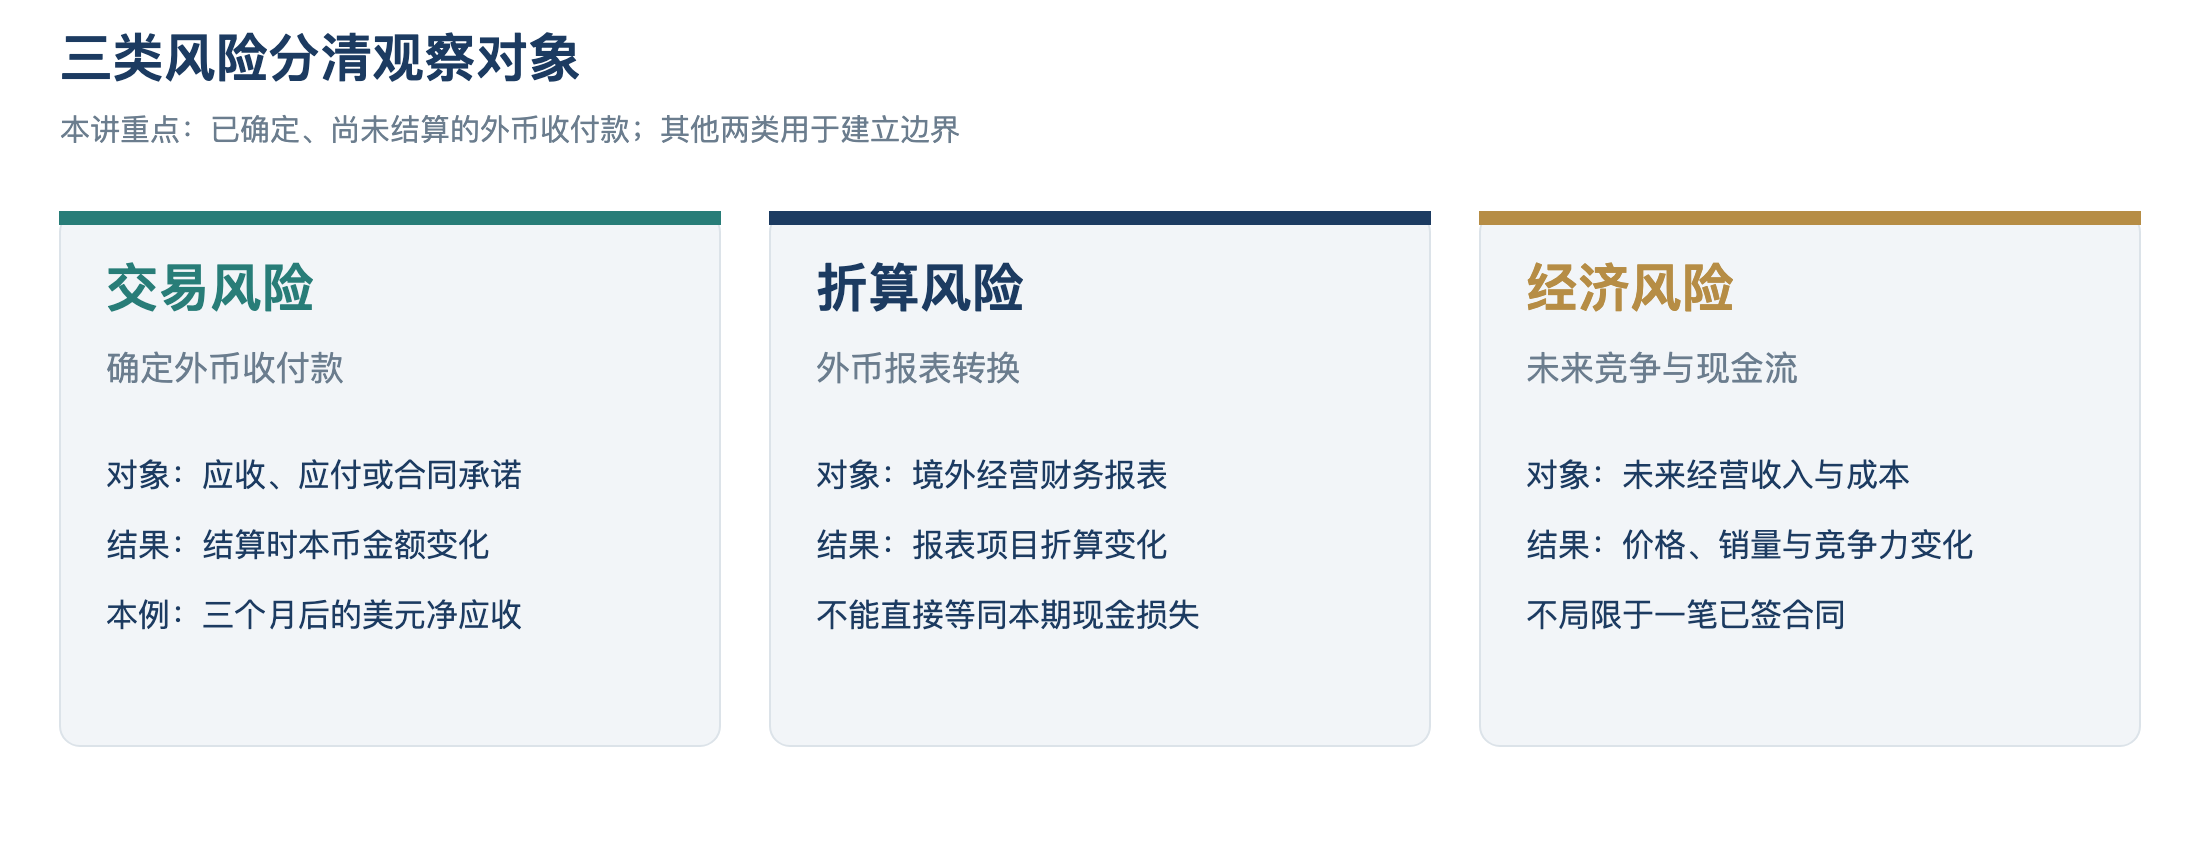
\includegraphics[width=.98\linewidth,height=7.3cm,keepaspectratio]{02_风险分类.png}\captionof{figure}{三类风险及本讲观察范围。依据教材第九章第一节整理。}\end{minipage}\par\addvspace{7pt}

\subsection*{业务清单的四项核对}

\begingroup\small\setstretch{1.10}\setlength{\tabcolsep}{6pt}\renewcommand{\arraystretch}{1.24}
\arrayrulecolor{Line}
\begin{longtable}{>{\raggedright\arraybackslash}p{\dimexpr0.15999\linewidth-2\tabcolsep\relax}>{\raggedright\arraybackslash}p{\dimexpr0.36003\linewidth-2\tabcolsep\relax}>{\raggedright\arraybackslash}p{\dimexpr0.47998\linewidth-2\tabcolsep\relax}}
\toprule[.8pt]\rowcolor{Navy}
\color{white}\bfseries 核对项 & \color{white}\bfseries 本例条件 & \color{white}\bfseries 条件变化时的处理 \\
\midrule\endfirsthead
\toprule[.8pt]\rowcolor{Navy}
\color{white}\bfseries 核对项 & \color{white}\bfseries 本例条件 & \color{white}\bfseries 条件变化时的处理 \\
\midrule\endhead
\midrule\multicolumn{3}{r}{\footnotesize\color{Muted}续下页}\\\endfoot
\bottomrule[.8pt]\endlastfoot
主体 & 同一企业可统一管理的现金流 & 不同法人或受限资金不能直接假定可自由轧差 \\
\midrule[.25pt]
\rowcolor{Pale}
币种 & 收付均为美元 & 不同币种需分别归集，不能直接相减 \\
\midrule[.25pt]
日期 & 均为三个月后同日结算 & 日期错配须分析融资、交割或滚动安排 \\
\midrule[.25pt]
\rowcolor{Pale}
确定性 & 收款与付款金额均已确定 & 预测订单变化时，须复核是否出现超额套保 \\
\midrule[.25pt]
\end{longtable}\endgroup

\subsection*{教学重点及突破方式}

重点是净敞口与交易安排的匹配，以及按事前目标评价套保效果。先画现金流，再按主体、币种、日期和确定性分桶；用共同参数完成三种比例、三个情景的同口径比较。

\subsection*{教学难点及突破方式}

难点是把“收入稳定”与“事后收入最高”区分开。先读情景曲线，再引入280万元下限，让学生用预算、机会收益和条件边界解释选择；不以预测汇率代替管理目标。

\clearpage
\section{从合同到预算的管理逻辑}\label{sec:risklogic}
\brief{先核实业务条件，再计量净敞口；由净方向决定工具安排，最后按事前预算评价方案。条件变化时，返回合同清单重新核对。}
\noindent\begin{minipage}{\linewidth}\centering
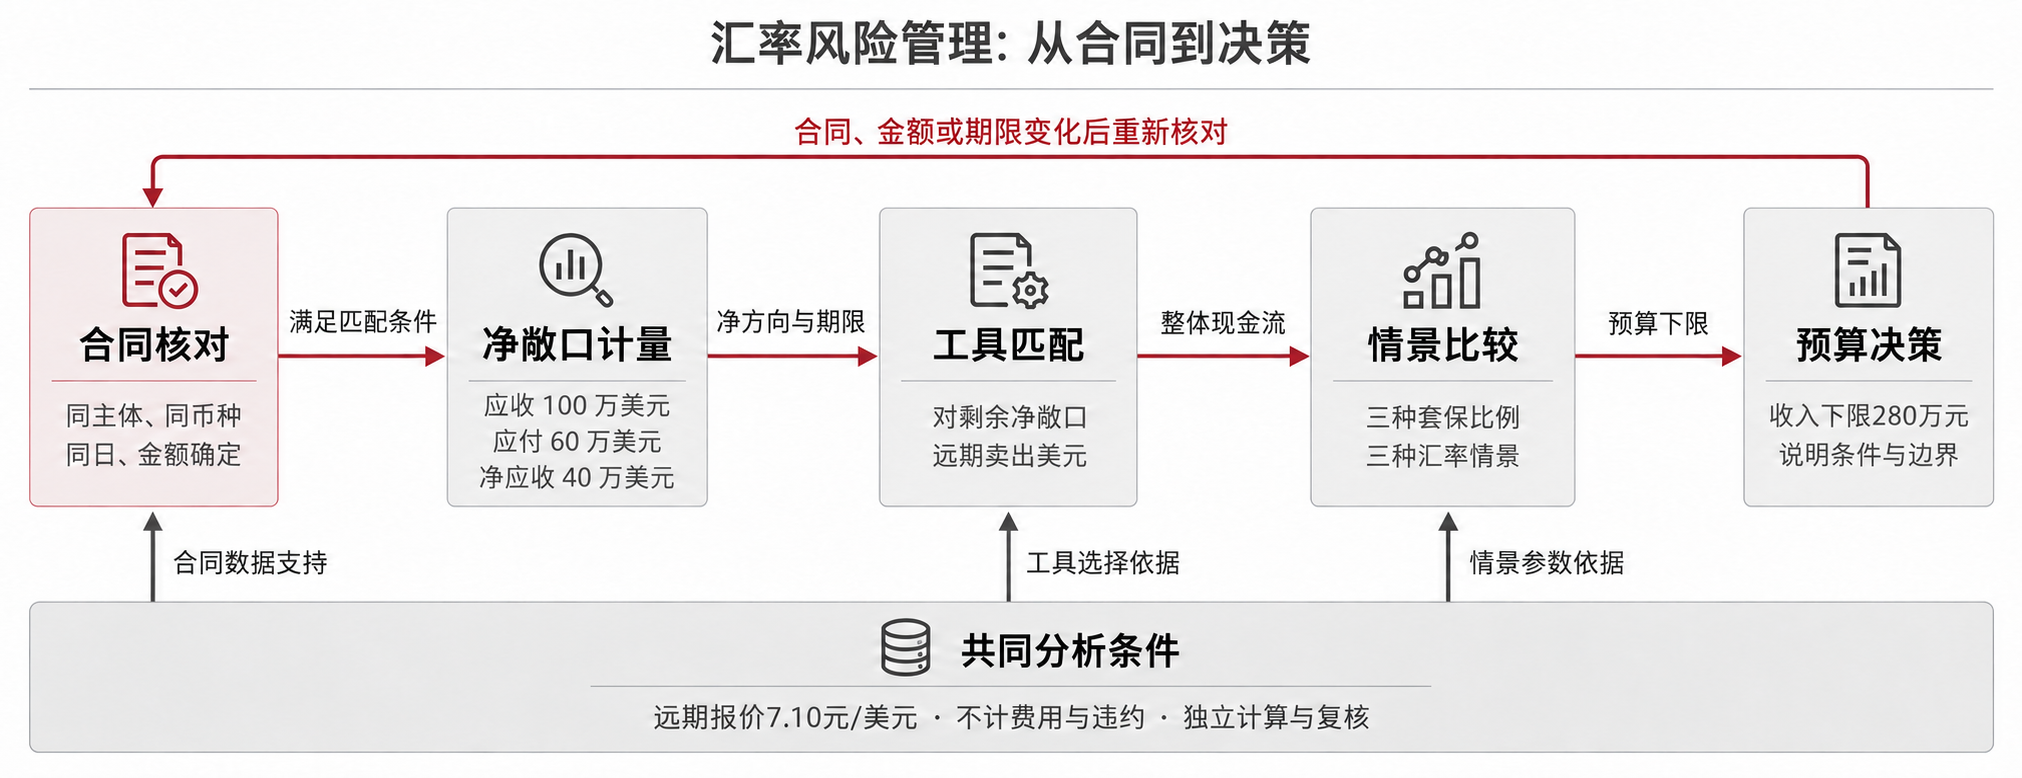
\includegraphics[width=\linewidth]{14_风险管理逻辑_Imagegen.png}
\captionof{figure}{合同核对、敞口计量、工具匹配、情景比较和预算决策构成相互衔接的管理链；上方回路表示条件变化后的重新核对。}
\end{minipage}
\subsection*{在互动网页中观察整体结果}
\noindent\begin{minipage}{\linewidth}\centering
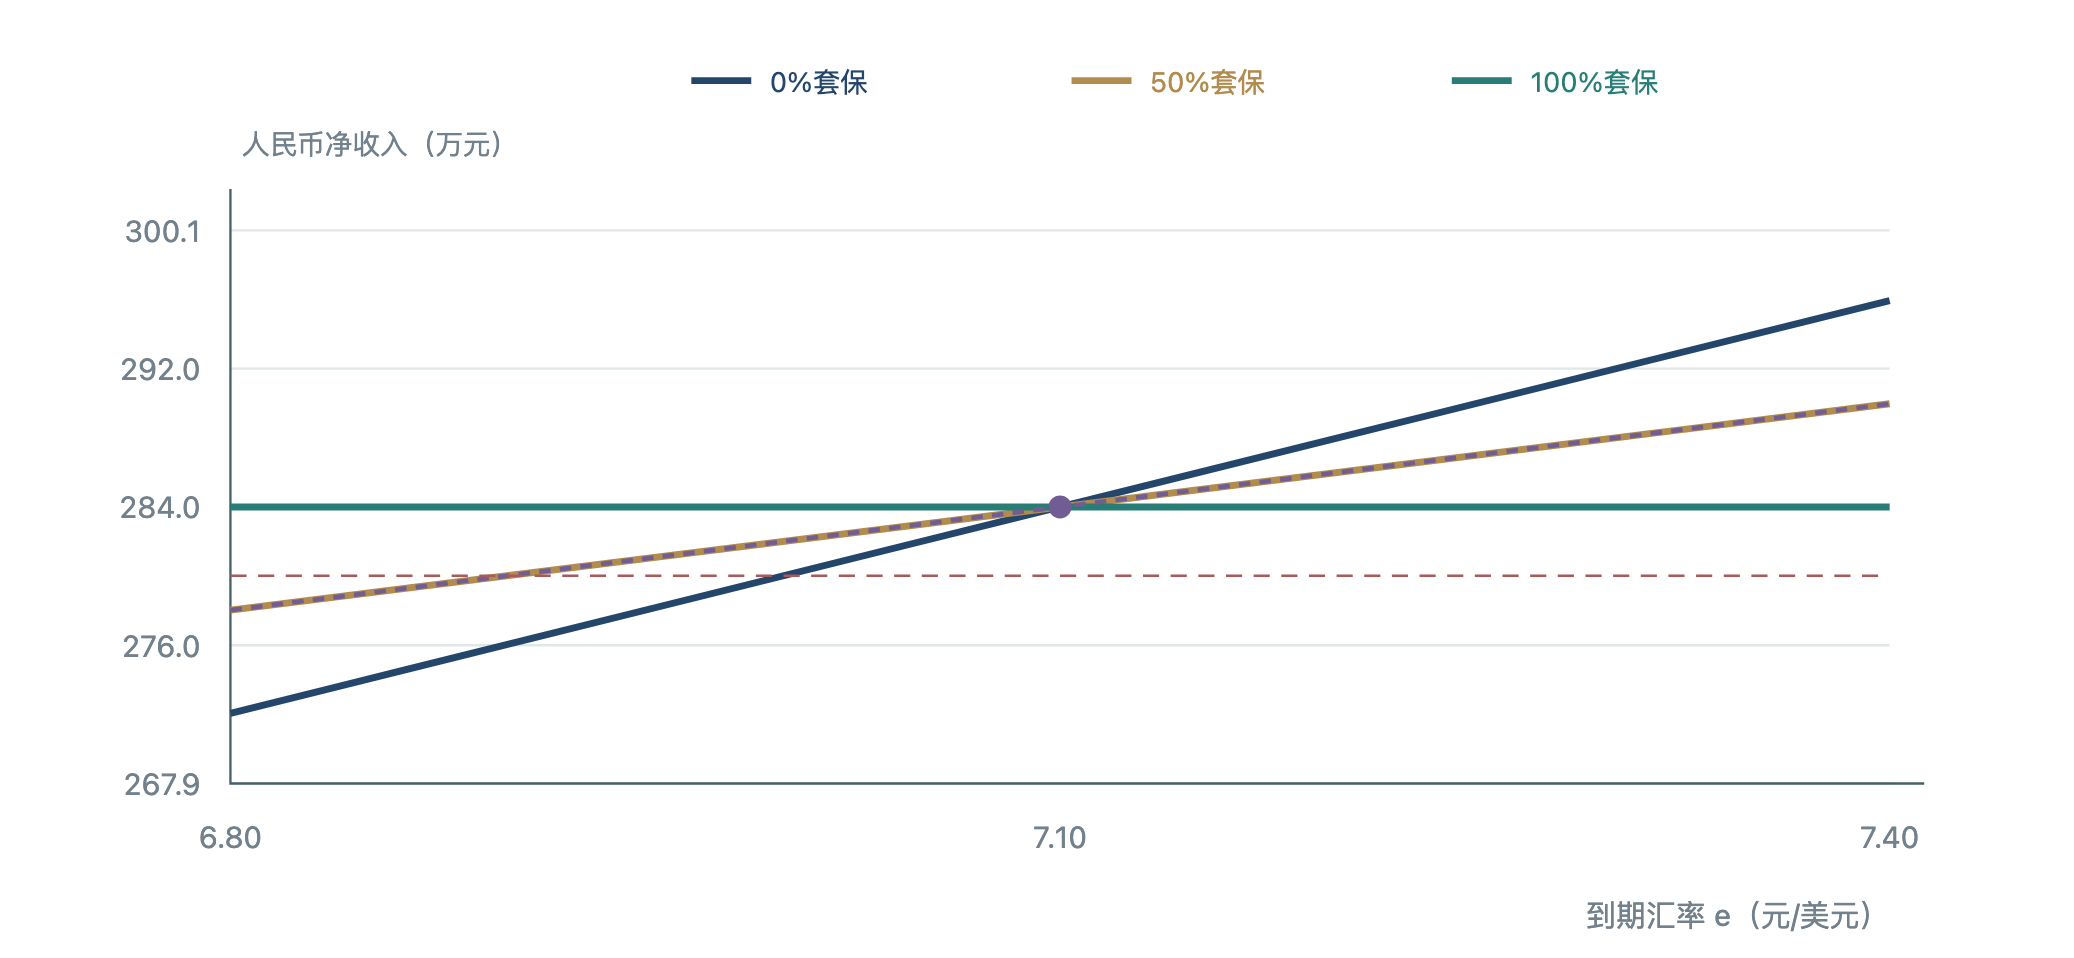
\includegraphics[width=.98\linewidth]{16_HTML情景曲线.png}
\captionof{figure}{配套GitHub Pages网页的实际曲线视图。图中的关系会随参数变化即时更新；截图仅用于展示计算结果，不表示真实的汇率时间路径，也不构成汇率预测。}
\end{minipage}
\hspace*{2em}当到期汇率为6.80时，不套保、50\%套保与100\%套保的净折算收入分别为272、278、284万元。收入下限为280万元时，三个离散方案中仅100\%套保达到该情景下限；完整评价仍须核对全部给定情景和业务条件。

条件变化时，应重新核查金额、日期、确定性与授权。套保的目标是管理不确定性，不承诺在事后获得最高折算收入。

\chapter{教学路径与课堂组织}\label{chap:path}

\section{教学方法与整体路径}\label{sec:g6}

教学方法、教学内容和教学目标逐项对应，保证各环节具有明确的学习任务与可观察的达成证据。

\par\addvspace{8pt}\noindent\begin{minipage}{\linewidth}\centering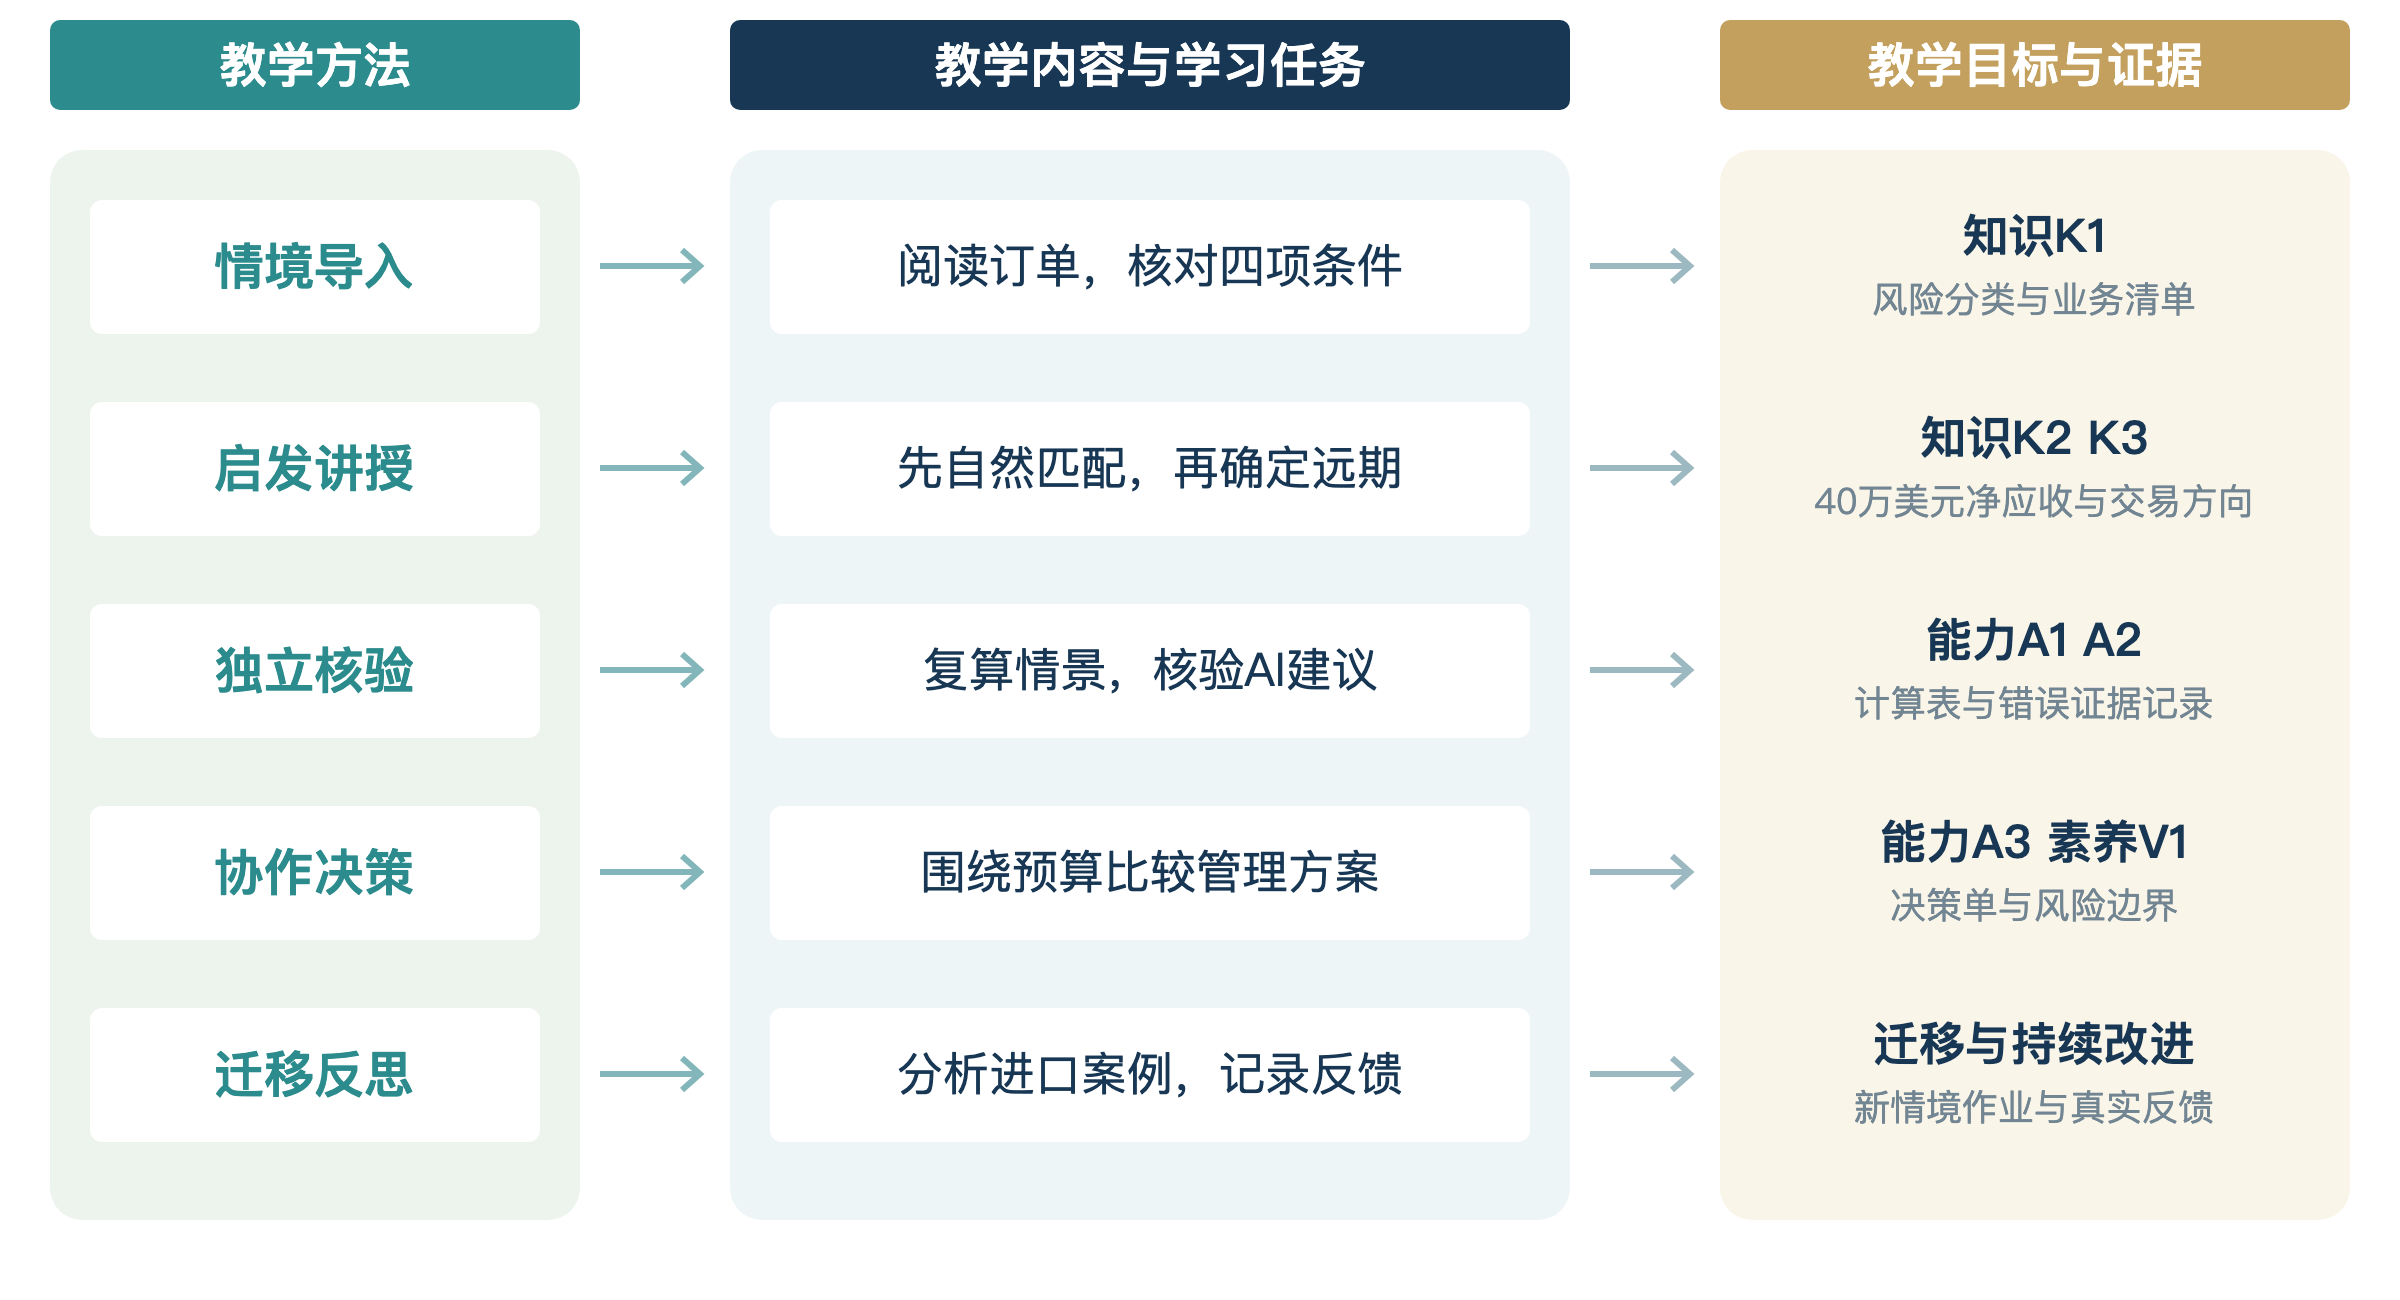
\includegraphics[width=.98\linewidth,height=8.2cm,keepaspectratio]{12_方法内容目标.png}\captionof{figure}{教学方法、学习任务与目标证据的对应关系。图形与任务结构为本讲原创。}\end{minipage}\par\addvspace{7pt}

\subsection*{方法选择及其适用环节}

\begingroup\small\setstretch{1.10}\setlength{\tabcolsep}{6pt}\renewcommand{\arraystretch}{1.24}
\arrayrulecolor{Line}
\begin{longtable}{>{\raggedright\arraybackslash}p{\dimexpr0.23999\linewidth-2\tabcolsep\relax}>{\raggedright\arraybackslash}p{\dimexpr0.76001\linewidth-2\tabcolsep\relax}}
\toprule[.8pt]\rowcolor{Navy}
\color{white}\bfseries 教学方式 & \color{white}\bfseries 具体安排与理由 \\
\midrule\endfirsthead
\toprule[.8pt]\rowcolor{Navy}
\color{white}\bfseries 教学方式 & \color{white}\bfseries 具体安排与理由 \\
\midrule\endhead
\midrule\multicolumn{2}{r}{\footnotesize\color{Muted}续下页}\\\endfoot
\bottomrule[.8pt]\endlastfoot
启发式讲授 & 从“每美元换多少人民币”和到期现金流出发，纠正标价、净额与工具方向的误解。 \\
\midrule[.25pt]
\rowcolor{Pale}
探究式核验 & 先完成个人计算，再审查预置的AI建议，提交错误识别结果、核验证据和修正意见，避免因表述流畅而直接采纳建议。 \\
\midrule[.25pt]
协作与非标准答案任务 & 围绕预算比较离散方案，允许提出其他比例，但须给出条件、计算与风险边界。 \\
\midrule[.25pt]
\rowcolor{Pale}
课前准备与课后迁移 & 用Q1—Q2诊断前置知识；课后迁移到美元净应付，检验方法能否跨情境使用。 \\
\midrule[.25pt]
\end{longtable}\endgroup

完整路径：课前诊断 \ensuremath{\rightarrow} 课堂识险与计算 \ensuremath{\rightarrow} AI核验与小组决策 \ensuremath{\rightarrow} 课末测验 \ensuremath{\rightarrow} 课后迁移与学习反馈。两学时各45分钟，课堂总计90分钟。

\clearpage

\section{教学过程 第一学时}\label{sec:g7}

0—45分钟：统一基本概念和计算口径，完成合同核对、净敞口计量和远期交易匹配，形成完整的计算流程。

\begingroup\small\setstretch{1.10}\setlength{\tabcolsep}{6pt}\renewcommand{\arraystretch}{1.24}
\arrayrulecolor{Line}
\begin{longtable}{>{\raggedright\arraybackslash}p{\dimexpr0.16997\linewidth-2\tabcolsep\relax}>{\raggedright\arraybackslash}p{\dimexpr0.10003\linewidth-2\tabcolsep\relax}>{\raggedright\arraybackslash}p{\dimexpr0.43001\linewidth-2\tabcolsep\relax}>{\raggedright\arraybackslash}p{\dimexpr0.29999\linewidth-2\tabcolsep\relax}}
\toprule[.8pt]\rowcolor{Navy}
\color{white}\bfseries 教学环节 & \color{white}\bfseries 用时 & \color{white}\bfseries 教学内容与师生活动 & \color{white}\bfseries 设计意图 \\
\midrule\endfirsthead
\toprule[.8pt]\rowcolor{Navy}
\color{white}\bfseries 教学环节 & \color{white}\bfseries 用时 & \color{white}\bfseries 教学内容与师生活动 & \color{white}\bfseries 设计意图 \\
\midrule\endhead
\midrule\multicolumn{4}{r}{\footnotesize\color{Muted}续下页}\\\endfoot
\bottomrule[.8pt]\endlastfoot
情境导入 & 0—5\par\noindent 5分钟 & 教师呈现订单、收付日期与预算任务，结合回信关于服务国家战略和西部发展的要求；学生说明稳健经营与订单履约的关系。 & 将价值要求融入专业任务，避免在计算结束后简单附加政治表述。 \\
\midrule[.25pt]
\rowcolor{Pale}
诊断回顾 & 5—12\par\noindent 7分钟 & 反馈课前 Q1、Q2；规范汇率表述（7.10元/美元即1美元换7.10元），并结合 6.80 的最新汇率，引导学生分析币值变动带来的影响。 & 诊断标价和风险分类，先纠正方向再进入计算。 \\
\midrule[.25pt]
风险识别与计量 & 12—25\par\noindent 13分钟 & 教师简析三类风险并示范合同清单；学生核对主体、币种、日期、确定性，并独立计算净应收（如100\ensuremath{-}60）。 & 用分桶清单减轻认知负荷；检查答案是否写清净应收、币种和日期。 \\
\midrule[.25pt]
\rowcolor{Pale}
自然匹配与远期 & 25—40\par\noindent 15分钟 & 先讲60万美元自然匹配，再讲40万美元远期卖出；学生完成0\%、50\%、100\%在6.80下的计算。 & 由业务现金流推导工具方向；强调不对自然匹配部分重复套保。 \\
\midrule[.25pt]
第一学时检验 & 40—45\par\noindent 5分钟 & 学生独立完成Q3、Q4后说明理由；教师核对净额和交易方向，并用两句话归纳。 & 形成个人学习证据；为第二学时AI核验建立正确基准。 \\
\midrule[.25pt]
\end{longtable}\endgroup

\subsection*{典型师生对话与反馈}

学生若说“收入100万美元，所以卖出100万美元”，教师提示：“同日应支付的60万美元用哪笔资金支付？”学生先在清单上圈出可匹配部分，再重新写净敞口。教师随后说明：若盲目卖出100万美元，可能形成60万美元超额套保。

第一学时结束应保留三项板书：四项核对、N=40万美元、远期卖出美元。学生没有掌握方向时，第二学时优先完成基本核验，不追加复杂比例推导。

\clearpage

\section{教学过程 第二学时}\label{sec:g8}

45—90分钟：在正确计算的基础上开展AI核验与预算决策。学生要用可复核的证据说明判断，而不能只给出一个套保比例。

\begingroup\small\setstretch{1.10}\setlength{\tabcolsep}{6pt}\renewcommand{\arraystretch}{1.24}
\arrayrulecolor{Line}
\begin{longtable}{>{\raggedright\arraybackslash}p{\dimexpr0.16997\linewidth-2\tabcolsep\relax}>{\raggedright\arraybackslash}p{\dimexpr0.10003\linewidth-2\tabcolsep\relax}>{\raggedright\arraybackslash}p{\dimexpr0.43001\linewidth-2\tabcolsep\relax}>{\raggedright\arraybackslash}p{\dimexpr0.29999\linewidth-2\tabcolsep\relax}}
\toprule[.8pt]\rowcolor{Navy}
\color{white}\bfseries 教学环节 & \color{white}\bfseries 用时 & \color{white}\bfseries 教学内容与师生活动 & \color{white}\bfseries 设计意图 \\
\midrule\endfirsthead
\toprule[.8pt]\rowcolor{Navy}
\color{white}\bfseries 教学环节 & \color{white}\bfseries 用时 & \color{white}\bfseries 教学内容与师生活动 & \color{white}\bfseries 设计意图 \\
\midrule\endhead
\midrule\multicolumn{4}{r}{\footnotesize\color{Muted}续下页}\\\endfoot
\bottomrule[.8pt]\endlastfoot
AI建议核验 & 45—57\par\noindent 12分钟 & 先个人复核3分钟，再同伴核对5分钟，最后教师归纳4分钟；依据AI核验单逐项标注错误、证据和修正。 & 将生成式AI使用转化为可评估的审查过程；检查是否出现“用AI证明AI”。 \\
\midrule[.25pt]
\rowcolor{Pale}
小组情景决策 & 57—72\par\noindent 15分钟 & 小组使用配套HTML网页比较三个情景和三种套保比例，以人民币净收入不低于280万元为目标形成决策单。基础组代入计算，提高组探索区间内h下限。 & 以预算约束引导学生分析和评价方案；每组至少记录一个不采纳的方案及其原因。 \\
\midrule[.25pt]
展示与教师点拨 & 72—82\par\noindent 10分钟 & 抽取两组各3分钟展示，教师4分钟综合点评；其余组提交书面成果。点评按正确性、证据、边界、表达展开。 & 通过公开论证促进同伴学习；不要求每组都进行现场汇报，以确保活动能在规定时间内完成。 \\
\midrule[.25pt]
\rowcolor{Pale}
课末测验与迁移 & 82—90\par\noindent 8分钟 & 4分钟完成Q5、Q6，2分钟归纳，2分钟布置进口企业迁移任务与退出反馈。 & 用个人结果检验目标达成，并将方法迁移到净应付情境。 \\
\midrule[.25pt]
\end{longtable}\endgroup

\subsection*{小组角色与产出}

建议每组4—6人，分别承担合同核对、计算、AI核验和汇报记录任务，人数较少时合并角色。提交一页决策单：净敞口、工具方向与期限、情景表、预算结论、风险边界与复核触发条件。

\subsection*{预算讨论的教师参考结论}

在0\%、50\%、100\%三个离散方案中，只有100\%套保在给定三个情景下均达到280万元下限。允许学生提出其他比例，但必须说明适用条件并验证计算结果；若要求到期汇率在6.80—7.40区间内的收入均不低于280万元，则最不利情景为6.80，由此可得h至少为2/3。该结论不构成对任意未来汇率情景的保证。

\subsection*{扫码进入互动任务}

三个互动任务共用访问密码：\texttt{scu1896}。

\begin{center}\begin{minipage}[t]{.31\linewidth}\centering\QRSlot{qr_risk_lab}{02}{情景实验}{\RiskLabURL}\par\smallskip{\bfseries\color{Navy}情景实验}\par{\footnotesize\color{Muted}调整比例与报价，动态比较结果}\end{minipage}\hfill\begin{minipage}[t]{.31\linewidth}\centering\QRSlot{qr_ai_review}{03}{AI核验}{\AIReviewURL}\par\smallskip{\bfseries\color{Navy}AI核验}\par{\footnotesize\color{Muted}记录错误、证据与修正}\end{minipage}\hfill\begin{minipage}[t]{.31\linewidth}\centering\QRSlot{qr_quiz_transfer}{04}{测验迁移}{\QuizTransferURL}\par\smallskip{\bfseries\color{Navy}测验迁移}\par{\footnotesize\color{Muted}四选一测验与进口案例}\end{minipage}\end{center}

\chapter{AI赋能与学习评价}\label{chap:assessment}

\section{AI赋能与算例核验}\label{sec:g9}

先用独立计算建立正确基准，再核验建议。预置文本仅用于核验练习，不作为真实AI工具的运行日志。联网使用时记录真实工具、时间、提示词和输出。

\begin{equation}N=100-60=40\quad\text{（万美元）}.\end{equation}

\begin{equation}R_h(e)=40\left[h\times7.10+(1-h)e\right]\quad\text{（万元人民币）}.\end{equation}

\begingroup\small\setstretch{1.10}\setlength{\tabcolsep}{6pt}\renewcommand{\arraystretch}{1.24}
\arrayrulecolor{Line}
\begin{longtable}{>{\raggedright\arraybackslash}p{\dimexpr0.25000\linewidth-2\tabcolsep\relax}>{\raggedright\arraybackslash}p{\dimexpr0.25000\linewidth-2\tabcolsep\relax}>{\raggedright\arraybackslash}p{\dimexpr0.25000\linewidth-2\tabcolsep\relax}>{\raggedright\arraybackslash}p{\dimexpr0.25000\linewidth-2\tabcolsep\relax}}
\toprule[.8pt]\rowcolor{Navy}
\color{white}\bfseries 到期汇率 & \color{white}\bfseries 0\%套保 & \color{white}\bfseries 50\%套保 & \color{white}\bfseries 100\%套保 \\
\midrule\endfirsthead
\toprule[.8pt]\rowcolor{Navy}
\color{white}\bfseries 到期汇率 & \color{white}\bfseries 0\%套保 & \color{white}\bfseries 50\%套保 & \color{white}\bfseries 100\%套保 \\
\midrule\endhead
\midrule\multicolumn{4}{r}{\footnotesize\color{Muted}续下页}\\\endfoot
\bottomrule[.8pt]\endlastfoot
6.80 & 272 & 278 & 284 \\
\midrule[.25pt]
\rowcolor{Pale}
7.10 & 284 & 284 & 284 \\
\midrule[.25pt]
7.40 & 296 & 290 & 284 \\
\midrule[.25pt]
\end{longtable}\endgroup

共同条件：同主体、同币种、同日且金额确定，忽略费用、融资、保证金占用、违约与税费。R为外币净收款的人民币折算金额，不等于企业利润。50\%套保在6.80下为20\ensuremath{\times}7.10+20\ensuremath{\times}6.80=278万元。

\par\addvspace{8pt}\noindent\begin{minipage}{\linewidth}\centering
\includegraphics[width=.98\linewidth,height=7.3cm,keepaspectratio]{06_AI核验路径_ElegantBook.pdf}\captionof{figure}{先独立判断，再核验与修正；完整提示词与填写表见附件二。 计算工具提供结果，AI提供待核建议，最终判断由学生与教师完成。}\end{minipage}\par\addvspace{7pt}

\begingroup\small\setstretch{1.10}\setlength{\tabcolsep}{6pt}\renewcommand{\arraystretch}{1.24}
\arrayrulecolor{Line}
\begin{longtable}{>{\raggedright\arraybackslash}p{\dimexpr0.23999\linewidth-2\tabcolsep\relax}>{\raggedright\arraybackslash}p{\dimexpr0.76001\linewidth-2\tabcolsep\relax}}
\toprule[.8pt]\rowcolor{Navy}
\color{white}\bfseries 核验焦点 & \color{white}\bfseries 必须给出的证据 \\
\midrule\endfirsthead
\toprule[.8pt]\rowcolor{Navy}
\color{white}\bfseries 核验焦点 & \color{white}\bfseries 必须给出的证据 \\
\midrule\endhead
\midrule\multicolumn{2}{r}{\footnotesize\color{Muted}续下页}\\\endfoot
\bottomrule[.8pt]\endlastfoot
基数与方向 & 100\ensuremath{-}60=40万美元净应收，应远期卖出美元。 \\
\midrule[.25pt]
\rowcolor{Pale}
预测与预算 & 6.80情景下，不套保的人民币净收入仅为272万元，低于280万元的预算下限，因此不能凭汇率预测认定不存在预算风险。 \\
\midrule[.25pt]
锁定与边界 & 完全套保可将本笔净应收的人民币折算收入锁定为284万元；到期汇率为7.40时，不套保的收入为296万元，因此完全套保不保证事后收入最高或企业利润最大。 \\
\midrule[.25pt]
\end{longtable}\endgroup

每类错误5分：识别2分、证据2分、修正1分，四类合计20分。可使用学校允许的联网AI工具；HTML仅用于确定性计算和可视化，不属于AI模型。

\clearpage
\section{从AI建议到可复核的课堂证据}\label{sec:ailogic}
\brief{先将AI建议视为待核验文本。学生独立完成计算后，再给出核验证据并提出修正意见。此页配合原定12分钟核验活动使用，不增加课堂时长。}
\noindent\begin{minipage}{\linewidth}\centering
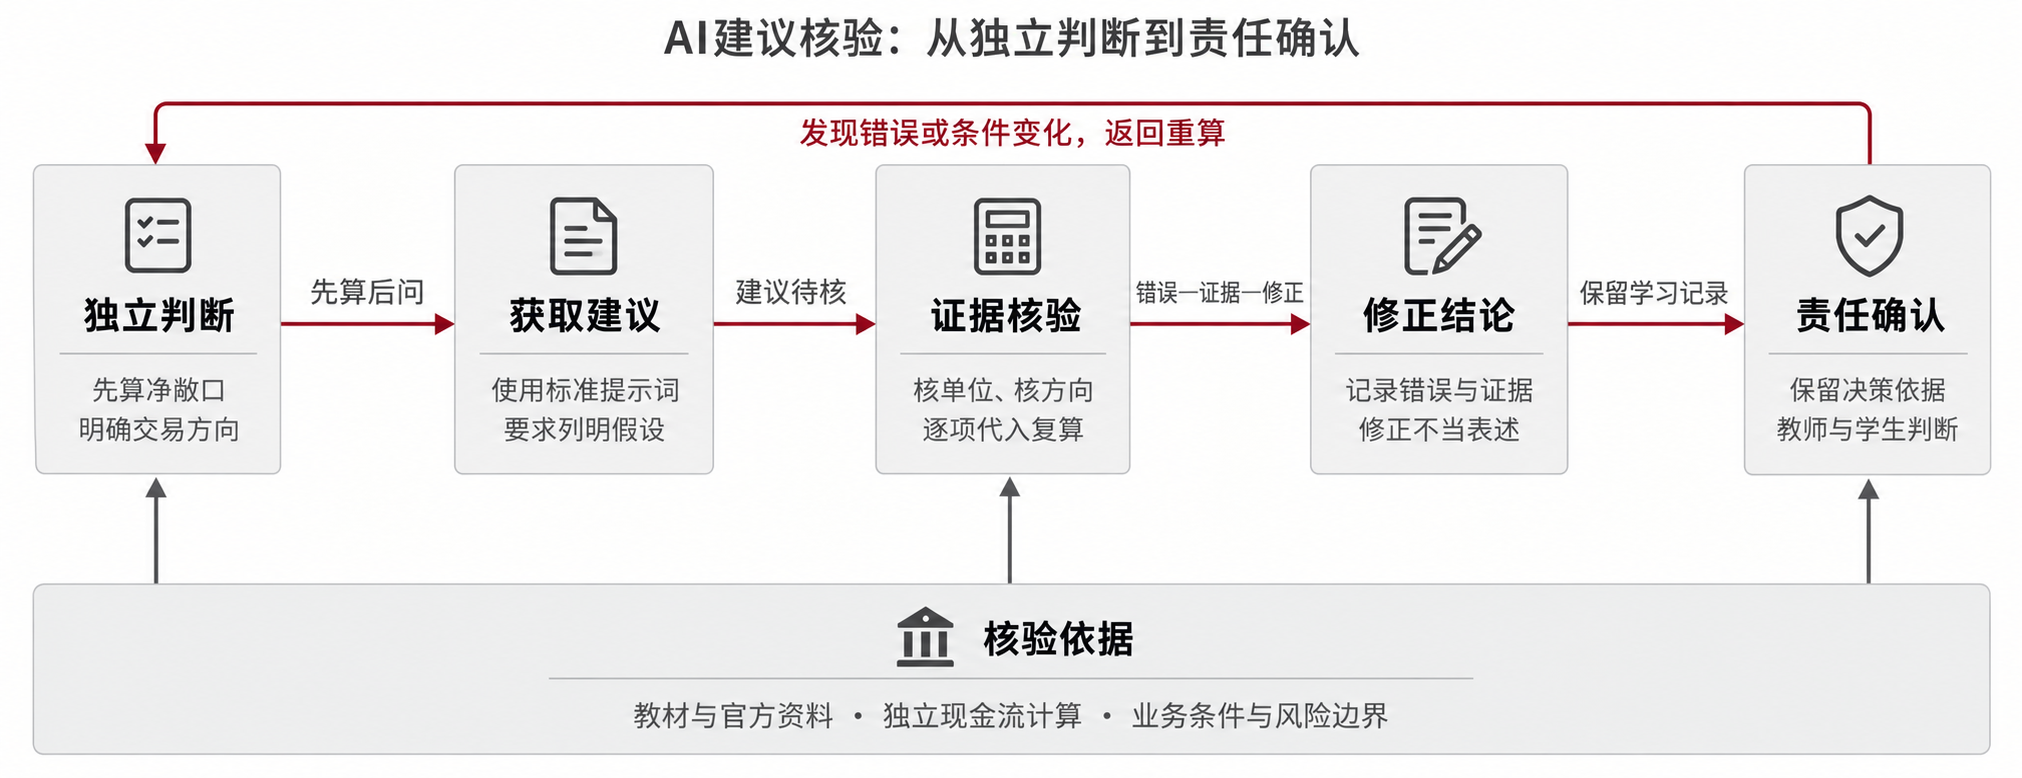
\includegraphics[width=\linewidth]{15_AI核验逻辑_Imagegen.png}
\captionof{figure}{核验依据支撑独立判断、证据核验与责任确认；发现错误或条件变化时返回重算。最终判断由教师与学生完成。}
\end{minipage}
\subsection*{将错误、证据与修正写在同一记录中}
\noindent\begin{minipage}{\linewidth}\centering

\includegraphics[width=.98\linewidth]{17_HTML核验单.png}
\captionof{figure}{配套互动网页中的核验单填写示例。该图展示操作与证据格式，不代表实际学生作答、成绩或教学成效。}
\end{minipage}
\hspace*{2em}本例先用100减去60，得到40万美元净应收，再据此确定应远期卖出美元。只说“AI错了”不能作为核验证据；修正后的结论必须说明主体、币种、日期和金额确定性等适用条件。

预置文本仅用于核验练习，不作为真实AI工具的运行日志。联网使用学校允许的工具时，另行记录实际提示词与输出。

\clearpage

\section{全过程考核与评价}\label{sec:g10}

本讲评价分为个人学习70分和小组决策30分，形成贯穿课前、课中和课后的连续评价证据，不改变整门课程原有的总评比例。

\begingroup\small\setstretch{1.10}\setlength{\tabcolsep}{6pt}\renewcommand{\arraystretch}{1.24}
\arrayrulecolor{Line}
\begin{longtable}{>{\raggedright\arraybackslash}p{\dimexpr0.24995\linewidth-2\tabcolsep\relax}>{\raggedright\arraybackslash}p{\dimexpr0.12005\linewidth-2\tabcolsep\relax}>{\raggedright\arraybackslash}p{\dimexpr0.63001\linewidth-2\tabcolsep\relax}}
\toprule[.8pt]\rowcolor{Navy}
\color{white}\bfseries 任务 & \color{white}\bfseries 分值 & \color{white}\bfseries 具体计分与证据 \\
\midrule\endfirsthead
\toprule[.8pt]\rowcolor{Navy}
\color{white}\bfseries 任务 & \color{white}\bfseries 分值 & \color{white}\bfseries 具体计分与证据 \\
\midrule\endhead
\midrule\multicolumn{3}{r}{\footnotesize\color{Muted}续下页}\\\endfoot
\bottomrule[.8pt]\endlastfoot
课前诊断与准备 & 10 & Q1、Q2各3分；合同清单准备4分。诊断后允许订正，保留初答与订正。 \\
\midrule[.25pt]
\rowcolor{Pale}
个人课堂计算与测验 & 20 & Q3、Q4各4分，Q5、Q6各3分；个人情景计算表6分。 \\
\midrule[.25pt]
AI核验记录 & 20 & 四类错误各5分：识别2、证据2、修正1。 \\
\midrule[.25pt]
\rowcolor{Pale}
小组决策单 & 30 & 按专业正确40\%、证据与推理30\%、风险边界20\%、表达10\%折算。 \\
\midrule[.25pt]
课后进口企业迁移 & 20 & 净额与方向5分；计算6分；预算结论5分；边界与来源4分。 \\
\midrule[.25pt]
\end{longtable}\endgroup

\subsection*{小组决策量规}

\begingroup\small\setstretch{1.10}\setlength{\tabcolsep}{6pt}\renewcommand{\arraystretch}{1.24}
\arrayrulecolor{Line}
\begin{longtable}{>{\raggedright\arraybackslash}p{\dimexpr0.23003\linewidth-2\tabcolsep\relax}>{\raggedright\arraybackslash}p{\dimexpr0.42996\linewidth-2\tabcolsep\relax}>{\raggedright\arraybackslash}p{\dimexpr0.34001\linewidth-2\tabcolsep\relax}}
\toprule[.8pt]\rowcolor{Navy}
\color{white}\bfseries 维度及分值 & \color{white}\bfseries 充分达成 & \color{white}\bfseries 需改进 \\
\midrule\endfirsthead
\toprule[.8pt]\rowcolor{Navy}
\color{white}\bfseries 维度及分值 & \color{white}\bfseries 充分达成 & \color{white}\bfseries 需改进 \\
\midrule\endhead
\midrule\multicolumn{3}{r}{\footnotesize\color{Muted}续下页}\\\endfoot
\bottomrule[.8pt]\endlastfoot
专业正确 12分 & 净额、方向、金额、日期、公式与单位一致 & 漏项、反向或单位混乱；按错误严重程度扣分 \\
\midrule[.25pt]
\rowcolor{Pale}
证据与推理 9分 & 提供完整情景表，并按预算比较方案 & 只报比例，缺计算或用预测替代依据 \\
\midrule[.25pt]
风险边界 6分 & 说明期限、确定性、费用及经营变化的复核要求 & 声称保证利润、风险清零或未列条件 \\
\midrule[.25pt]
\rowcolor{Pale}
表达 3分 & 结论简洁，图表可复算，角色和记录清楚 & 结论与证据不对应或读者无法复算 \\
\midrule[.25pt]
\end{longtable}\endgroup

\subsection*{价值与专业评价相互支撑}

诚信体现在不隐藏不利情景、不编造AI记录；敬业体现在按合同与预算开展审慎分析；责任体现在说明调整条件和授权边界。评分应以上述行为证据为依据，不能以口号多少代替对专业表现的评价。

\clearpage

\section{教学反思与实施保障}\label{sec:g11}

本讲围绕报价方向、净敞口、工具匹配与预算解释设置观察点，以课堂作答、计算表和小组方案诊断学习困难，并据此调整教学节奏。

\begingroup\small\setstretch{1.10}\setlength{\tabcolsep}{6pt}\renewcommand{\arraystretch}{1.24}
\arrayrulecolor{Line}
\begin{longtable}{>{\raggedright\arraybackslash}p{\dimexpr0.28004\linewidth-2\tabcolsep\relax}>{\raggedright\arraybackslash}p{\dimexpr0.36999\linewidth-2\tabcolsep\relax}>{\raggedright\arraybackslash}p{\dimexpr0.34997\linewidth-2\tabcolsep\relax}}
\toprule[.8pt]\rowcolor{Navy}
\color{white}\bfseries 可能出现的问题 & \color{white}\bfseries 课堂调整 & \color{white}\bfseries 授课后核验依据 \\
\midrule\endfirsthead
\toprule[.8pt]\rowcolor{Navy}
\color{white}\bfseries 可能出现的问题 & \color{white}\bfseries 课堂调整 & \color{white}\bfseries 授课后核验依据 \\
\midrule\endhead
\midrule\multicolumn{3}{r}{\footnotesize\color{Muted}续下页}\\\endfoot
\bottomrule[.8pt]\endlastfoot
报价方向误判较多 & 增加“1美元换多少人民币”的单位解释，先暂缓h推导 & Q1初答与订正分布、学生解释记录 \\
\midrule[.25pt]
\rowcolor{Pale}
净额或方向仍不牢固 & 返回合同清单与远期现金流图，减少提高题 & Q3、Q4错因与个人计算表 \\
\midrule[.25pt]
小组用预测代替预算 & 要求提交最低收入和不采纳方案的证据 & 决策单的情景完整性、预算解释 \\
\midrule[.25pt]
\rowcolor{Pale}
AI核验仅停留在口头指出错误 & 教师示范一条“错误—证据—修正”，再让学生独立写其余 & 核验单证据栏的得分与引用质量 \\
\midrule[.25pt]
网络或设备不可用 & 使用离线HTML与纸质情景表，发放预置文本 & 任务完成情况及后备方案使用记录 \\
\midrule[.25pt]
\end{longtable}\endgroup

\subsection*{设计中值得保留的做法}

一组共同参数贯穿净额、套保、AI核验和预算决策，减少重复读题负担；个人先算、小组再议，防止少数学生包办；由现金流推导工具方向，再用情景比较检验方案，便于追踪错误来源。通过个人计算、同伴讨论与方案展示相互印证，形成可追踪的学习证据。

\subsection*{课后反思的写作路径}

按“观察到的事实—可能原因—采取的调整—下一次验证”记录。优先分析学生为什么漏掉应付款、为什么把预测当依据、为什么用事后最高收入评价套保。结合匿名反馈与作答记录分析共性错因，形成下一轮教学调整依据。

\subsection*{后续改进的触发条件}

若净额与方向仍出现同类错误，下次优先增加分桶练习；若计算正确但预算解释不足，增加两个目标不同的企业情景；若AI核验缺少证据，则缩短待核验的AI文本，强化来源定位与手算对照。教学改进应依据学生的具体错误、任务表现和评价结果展开。

\chapter{配套资源与资料依据}\label{chap:resources}

通过配套课件中的净敞口图与情景曲线，展示教案在课堂中的具体实施方式。完整主课件共26页，独立单选题共14页，二者均采用与本教案一致的案例参数和评价依据。

\par\addvspace{8pt}\noindent\begin{minipage}{\linewidth}\centering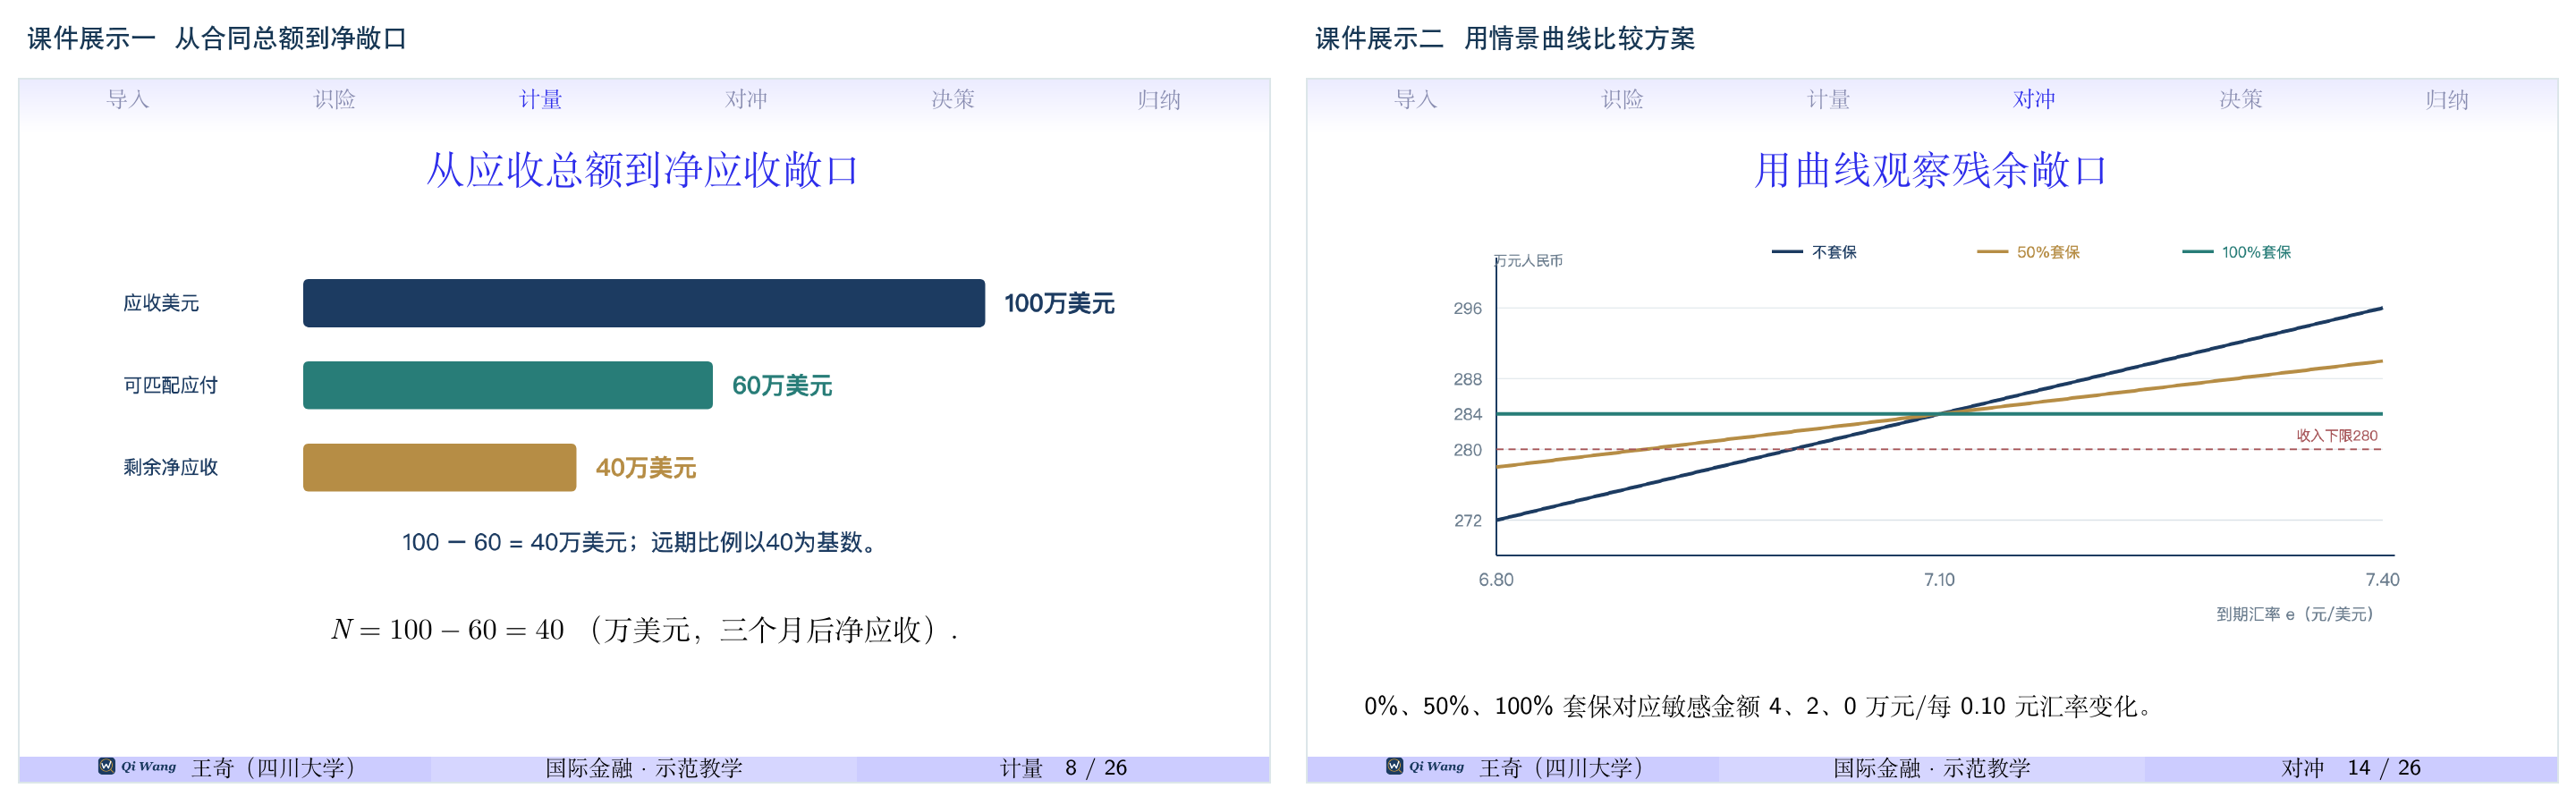
\includegraphics[width=.98\linewidth,height=7.3cm,keepaspectratio]{13_配套课件展示.png}\captionof{figure}{配套课件截图：从合同总额到净敞口，再以情景曲线解释稳定性与机会收益。}\end{minipage}\par\addvspace{7pt}

\subsection*{材料来源与使用范围}

{\small\setstretch{1.1}[1] 范小云、陈平主编：《国际金融》第二版，高等教育出版社，2019，第九章第一节，第256—266页。}

{\small\setstretch{1.1}[2] 习近平给四川大学全体师生的回信，2026年9月28日；教育部网站2026年9月29日刊载。\par{\footnotesize\url{https://www.moe.gov.cn/jyb_xwfb/moe_176/202609/t20260929_1452614.html}}}

{\small\setstretch{1.1}[3] 生态环境部转载新华社报道，2026年9月29日，可交叉核验回信主要表述。\par{\footnotesize\url{https://www.mee.gov.cn/ywdt/szyw/202609/t20260929_1175502.shtml}}}

{\small\setstretch{1.1}[4] 国家外汇管理局企业汇率风险管理服务小组：《企业汇率风险管理指引（2024年版）》。\par{\footnotesize\url{https://www.safe.gov.cn/hubei/file/file/20250627/70d7b5f7233246e89c92c8483bc446d9.pdf}}}

{\small\setstretch{1.1}[5] 国家外汇管理局四川省分局公开材料：《汇率风险中性基础知识》，2022年。用于风险中性概念，不作为当期业务规则。\par{\footnotesize\url{https://www.safe.gov.cn/sichuan/file/file/20220601/9ecf217f2bcd4812b32f41f44939e1b5.pdf}}}

\appendix\chapter{学习任务与评价附件}\label{chap:appendix}

\section{合同与净敞口任务单}\label{sec:g13}

学生姓名\rule{2cm}{.3pt}  学号\rule{2cm}{.3pt}  小组\rule{2cm}{.3pt}  日期\rule{2cm}{.3pt}

案例：西部某装备制造企业将在三个月后的同一天收取100万美元、支付60万美元，两笔金额均已确定。两笔现金流属于同一企业、币种均为美元。远期结汇报价7.10元/美元。完成核对后，再选择是否以及如何套保。

\begingroup\small\setstretch{1.10}\setlength{\tabcolsep}{6pt}\renewcommand{\arraystretch}{1.24}
\arrayrulecolor{Line}
\begin{longtable}{>{\raggedright\arraybackslash}p{\dimexpr0.18002\linewidth-2\tabcolsep\relax}>{\raggedright\arraybackslash}p{\dimexpr0.39998\linewidth-2\tabcolsep\relax}>{\raggedright\arraybackslash}p{\dimexpr0.42000\linewidth-2\tabcolsep\relax}}
\toprule[.8pt]\rowcolor{Navy}
\color{white}\bfseries 核对项 & \color{white}\bfseries 我核实的事实 & \color{white}\bfseries 若事实变化需补充的信息 \\
\midrule\endfirsthead
\toprule[.8pt]\rowcolor{Navy}
\color{white}\bfseries 核对项 & \color{white}\bfseries 我核实的事实 & \color{white}\bfseries 若事实变化需补充的信息 \\
\midrule\endhead
\midrule\multicolumn{3}{r}{\footnotesize\color{Muted}续下页}\\\endfoot
\bottomrule[.8pt]\endlastfoot
主体 & \rule{0pt}{9mm} & \rule{0pt}{9mm} \\
\midrule[.25pt]
\rowcolor{Pale}
币种 & \rule{0pt}{9mm} & \rule{0pt}{9mm} \\
\midrule[.25pt]
日期 & \rule{0pt}{9mm} & \rule{0pt}{9mm} \\
\midrule[.25pt]
\rowcolor{Pale}
确定性 & \rule{0pt}{9mm} & \rule{0pt}{9mm} \\
\midrule[.25pt]
\end{longtable}\endgroup

\subsection*{独立计算与解释}

净敞口算式：\hrulefill{}

净方向、币种与日期：\hrulefill{}

合适的远期交易方向及理由：\hrulefill{}

\begingroup\small\setstretch{1.10}\setlength{\tabcolsep}{6pt}\renewcommand{\arraystretch}{1.24}
\arrayrulecolor{Line}
\begin{longtable}{>{\raggedright\arraybackslash}p{\dimexpr0.25000\linewidth-2\tabcolsep\relax}>{\raggedright\arraybackslash}p{\dimexpr0.25000\linewidth-2\tabcolsep\relax}>{\raggedright\arraybackslash}p{\dimexpr0.25000\linewidth-2\tabcolsep\relax}>{\raggedright\arraybackslash}p{\dimexpr0.25000\linewidth-2\tabcolsep\relax}}
\toprule[.8pt]\rowcolor{Navy}
\color{white}\bfseries 到期汇率 & \color{white}\bfseries 0\%套保 & \color{white}\bfseries 50\%套保 & \color{white}\bfseries 100\%套保 \\
\midrule\endfirsthead
\toprule[.8pt]\rowcolor{Navy}
\color{white}\bfseries 到期汇率 & \color{white}\bfseries 0\%套保 & \color{white}\bfseries 50\%套保 & \color{white}\bfseries 100\%套保 \\
\midrule\endhead
\midrule\multicolumn{4}{r}{\footnotesize\color{Muted}续下页}\\\endfoot
\bottomrule[.8pt]\endlastfoot
6.80 & \rule{0pt}{9mm} & \rule{0pt}{9mm} & \rule{0pt}{9mm} \\
\midrule[.25pt]
\rowcolor{Pale}
7.10 & \rule{0pt}{9mm} & \rule{0pt}{9mm} & \rule{0pt}{9mm} \\
\midrule[.25pt]
7.40 & \rule{0pt}{9mm} & \rule{0pt}{9mm} & \rule{0pt}{9mm} \\
\midrule[.25pt]
\end{longtable}\endgroup

我采用的金额单位：\rule{2cm}{.3pt}  套保比例的计算基数：\rule{2cm}{.3pt}

同日匹配条件不成立时，为什么不能直接沿用40万美元这一净敞口计算结果？\par\noindent \hrulefill{}\par\noindent \hrulefill{}

作答要求：先个人完成，再参与讨论；计算表需保留至少一行代入过程。

\clearpage

\section{AI建议核验单}\label{sec:g14}

姓名\rule{2cm}{.3pt}  小组\rule{2cm}{.3pt}  使用方式：联网工具 / 预置文本（圈选）

实际联网使用时填写：工具名称\rule{2cm}{.3pt} 日期时间\rule{2cm}{.3pt}；附真实输出。使用预置文本时无需虚填工具或运行时间。

\begingroup\small\setstretch{1.10}\setlength{\tabcolsep}{6pt}\renewcommand{\arraystretch}{1.24}
\arrayrulecolor{Line}
\begin{longtable}{>{\raggedright\arraybackslash}p{\dimexpr0.37999\linewidth-2\tabcolsep\relax}>{\raggedright\arraybackslash}p{\dimexpr0.37003\linewidth-2\tabcolsep\relax}>{\raggedright\arraybackslash}p{\dimexpr0.24997\linewidth-2\tabcolsep\relax}}
\toprule[.8pt]\rowcolor{Navy}
\color{white}\bfseries 待核验文本 & \color{white}\bfseries 错误与复算证据 & \color{white}\bfseries 修正 \\
\midrule\endfirsthead
\toprule[.8pt]\rowcolor{Navy}
\color{white}\bfseries 待核验文本 & \color{white}\bfseries 错误与复算证据 & \color{white}\bfseries 修正 \\
\midrule\endhead
\midrule\multicolumn{3}{r}{\footnotesize\color{Muted}续下页}\\\endfoot
\bottomrule[.8pt]\endlastfoot
1. 公司应按100万美元全部套保，不需要考虑60万美元应付款。 & \rule{0pt}{16mm} & \rule{0pt}{16mm} \\
\midrule[.25pt]
\rowcolor{Pale}
2. 收到美元后担心人民币升值，应远期买入40万美元。 & \rule{0pt}{16mm} & \rule{0pt}{16mm} \\
\midrule[.25pt]
3. AI判断三个月后一定到7.40，因此不套保不会有预算风险。 & \rule{0pt}{16mm} & \rule{0pt}{16mm} \\
\midrule[.25pt]
\rowcolor{Pale}
4. 100\%远期套保可以保证企业利润最高，并消除所有风险。 & \rule{0pt}{16mm} & \rule{0pt}{16mm} \\
\midrule[.25pt]
\end{longtable}\endgroup

\subsection*{可复制的标准提示词}

你是企业财务分析助手。企业将在三个月后的同一天收取100万美元、支付60万美元，两笔金额均已确定，远期结汇7.10元/美元。请先核对主体、币种、日期与确定性，再计算净敞口，比较0\%、50\%、100\%套保在6.80、7.10、7.40下的人民币净收入。以万元人民币为单位列示公式和计算过程，说明交易方向、假设、预算目标以及结论的适用条件和局限。不预测汇率，不承诺利润最大化；对不确定的内容，先列出需要核实的信息。

每项5分：识别2分、证据2分、修正1分。正文“AI赋能与算例核验”及教师答案提供核验锚点。预置文本包含有意设置的错误，不代表专业结论或实时AI输出。

\clearpage

\section{小组风险管理决策单}\label{sec:g15}

小组\rule{2cm}{.3pt}  合同核对\rule{2cm}{.3pt}  计算\rule{2cm}{.3pt}  核验\rule{2cm}{.3pt}  汇报记录\rule{2cm}{.3pt}

任务：在本讲给定情景下，使三个月后的人民币净收入不低于280万元。比较0\%、50\%、100\%三个方案，写出可以复核的建议。

\begingroup\small\setstretch{1.10}\setlength{\tabcolsep}{6pt}\renewcommand{\arraystretch}{1.24}
\arrayrulecolor{Line}
\begin{longtable}{>{\raggedright\arraybackslash}p{\dimexpr0.34001\linewidth-2\tabcolsep\relax}>{\raggedright\arraybackslash}p{\dimexpr0.65999\linewidth-2\tabcolsep\relax}}
\toprule[.8pt]\rowcolor{Navy}
\color{white}\bfseries 决策要素 & \color{white}\bfseries 小组填写 \\
\midrule\endfirsthead
\toprule[.8pt]\rowcolor{Navy}
\color{white}\bfseries 决策要素 & \color{white}\bfseries 小组填写 \\
\midrule\endhead
\midrule\multicolumn{2}{r}{\footnotesize\color{Muted}续下页}\\\endfoot
\bottomrule[.8pt]\endlastfoot
净敞口及核对条件 & \rule{0pt}{9mm} \\
\midrule[.25pt]
\rowcolor{Pale}
远期方向、金额与交割日 & \rule{0pt}{9mm} \\
\midrule[.25pt]
所选方案与人民币结果 & \rule{0pt}{9mm} \\
\midrule[.25pt]
\rowcolor{Pale}
未采纳的方案及原因 & \rule{0pt}{9mm} \\
\midrule[.25pt]
采用的证据或数据来源 & \rule{0pt}{9mm} \\
\midrule[.25pt]
\rowcolor{Pale}
不能保证的结果与其他风险 & \rule{0pt}{9mm} \\
\midrule[.25pt]
经营变化后的复核触发条件 & \rule{0pt}{9mm} \\
\midrule[.25pt]
\end{longtable}\endgroup

\subsection*{简短决策陈述}

我们建议\hrulefill{}\par\noindent 原因与预算依据\hrulefill{}\par\noindent 在以下条件下需要重新评估\hrulefill{}

\subsection*{提高任务  可选}

若允许h在0—1之间连续变化，并要求到期汇率处于6.80—7.40区间时人民币净收入均不低于280万元，求h的下限，并说明为什么这一结论不能保证在任意未来汇率下都达到该收入目标。\par\noindent \hrulefill{}\par\noindent \hrulefill{}

评分30分：专业正确12分、证据推理9分、风险边界6分、表达3分。两组现场展示，其余提交书面记录。

\clearpage

\section{课前与课中四选一测验}\label{sec:g16}

\begingroup\small\setstretch{1.14}\setlength{\parskip}{3pt}
每题只有一个正确答案。Q1—Q2课前完成并订正，Q3—Q4在第一学时末独立完成。

\subsection*{Q1  课前诊断}

采用“元人民币/美元”报价，汇率由7.10降至6.80。在本讲条件下，正确的判断是。

A. 人民币贬值，美元净应收折算收入增加

B. 人民币升值，美元净应收折算收入减少

C. 美元升值，美元净应收折算收入减少

D. 人民币升值，美元净应收金额自动减少

\subsection*{Q2  课前诊断}

企业已签订合同，三个月后确定收取一笔美元货款，其人民币折算金额随汇率变化。这首先属于。

A. 境外报表折算风险

B. 国内商品库存数量风险

C. 外汇交易风险

D. 人民币现金存款利率风险

\subsection*{Q3  课中检验}

企业同日确定收取100万美元、支付60万美元，无其他外汇业务。自然匹配后的美元净敞口是。

A. 净应收40万美元

B. 净应收100万美元

C. 净应付60万美元

D. 净应收160万美元

\subsection*{Q4  课中检验}

对Q3中已确定的净敞口进行100\%远期套保，且期限匹配，企业应办理哪项交易？（　）

A. 远期买入100万美元

B. 远期卖出100万美元

C. 远期买入40万美元

D. 远期卖出40万美元

初答：Q1\_\_\_\_ Q2\_\_\_\_ Q3\_\_\_\_ Q4\_\_\_\_    订正：Q1\_\_\_\_ Q2\_\_\_\_\par\noindent 保留原答案；订正时，写明在汇率方向、风险分类、净额计算或交易安排方面的具体错误。
\endgroup

\clearpage

\section{课末测验与迁移作业}\label{sec:g17}

课末Q5—Q6个人独立完成。课后任务先判断净方向，再选择交易方向，不照搬出口企业的远期卖出安排。

\subsection*{Q5  课末测验}

企业有40万美元净应收，其中50\%按7.10元/美元的汇率远期结汇，其余在到期时按6.80元/美元结汇。忽略费用，人民币净收入是多少？（　）

A. 272万元

B. 278万元

C. 284万元

D. 296万元

\subsection*{Q6  课末测验}

在本讲确定净应收、忽略费用的条件下，对100\%远期套保的评价，最恰当的是。

A. 保证所有情景下收入最高

B. 保证企业全部经营利润不变

C. 锁定该笔净敞口的折算收入，但不保证事后收入最高

D. 只要AI预测人民币贬值，就应取消已确定的套保方案

\subsection*{课后任务  进口企业的美元净应付}

企业三个月后同日确定支付80万美元、收取30万美元。远期购汇7.12元/美元。到期汇率为6.90、7.12、7.40，忽略与主案例相同的成本及违约因素。企业希望人民币净付款成本在这些情景下不超过360万元。

提交一页分析：①按四项条件核对净敞口；②确定远期方向；③列出0\%、50\%、100\%套保成本；④选择满足预算的方案；⑤说明边界和经营变化后的复核要求。提高任务：求给定区间内最低h。

提交要求：计算过程与结论可复算；如使用AI，附实际提示词与核验记录，不以AI回答代替个人解释。建议课后48小时内提交，实际时间由教师发布。

\clearpage

\section{教师参考答案与错因}\label{sec:g18}

\begingroup\small\setstretch{1.14}\setlength{\parskip}{3pt}
正确答案依次为B、C、A、D、B、C。解析用于讲评与反馈；正式测验时不提前展示。

Q1  答案 B

A. 本币/外币报价下降表示人民币升值，方向判断反了。

B. 每美元换得的人民币减少；在美元净应收不变时，人民币收入减少。

C. 报价下降表示美元相对人民币贬值，而非升值。

D. 汇率改变折算金额，不自动改变合同规定的美元金额。

Q2  答案 C

A. 报表折算风险主要涉及外币财务报表的折算，与本题中已确定但尚未结算的外币收款无直接关系。

B. 本题没有商品库存数量变化，不能用它解释汇率引起的折算变化。

C. 已确定、尚未结算的外币收付款面临汇率变动，属于交易风险。

D. 题干未涉及人民币存款利率变化。

Q3  答案 A

A. 相同主体、币种和日期下，100\ensuremath{-}60=40万美元，为净应收。

B. 只计应收，漏掉可匹配的同日应付。

C. 忽略了金额更大的应收，将净方向判断反了。

D. 把流入与流出直接相加，得到的不是净敞口。

Q4  答案 D

A. 美元净应收需要卖出美元；买入100万美元会扩大美元多头。

B. 自然匹配后仅剩40万美元；卖出100万美元可能造成60万美元超额套保。

C. 买入美元适合匹配净应付，本题方向相反。

D. 按剩余40万美元净应收、同到期日远期卖出美元，方向与规模匹配。

Q5  答案 B

A. 272=40\ensuremath{\times}6.80，对应完全不套保。

B. 278=20\ensuremath{\times}7.10+20\ensuremath{\times}6.80，单位为万元人民币。

C. 284=40\ensuremath{\times}7.10，对应100\%远期套保。

D. 296=40\ensuremath{\times}7.40，是另一情景下不套保的结果。

Q6  答案 C

A. 当到期汇率高于7.10，不套保的折算收入可能更高。

B. 套保只能管理本笔交易的汇率不确定性，不能消除生产、信用等全部经营风险。

C. 在上述条件成立时锁定284万元；评价应结合预算目标和整体业务，不应只以事后最高收益为标准。

D. 预测不能替代风险目标；经营变化需要复核敞口、授权和调整成本。
\endgroup

\clearpage

\section{评分记录与迁移参考}\label{sec:g19}

按本讲量规记录成绩，保留个体与小组证据。评分记录与学生个人信息仅在授权教学环境中使用。

\begingroup\small\setstretch{1.10}\setlength{\tabcolsep}{6pt}\renewcommand{\arraystretch}{1.24}
\arrayrulecolor{Line}
\begin{longtable}{>{\raggedright\arraybackslash}p{\dimexpr0.36996\linewidth-2\tabcolsep\relax}>{\raggedright\arraybackslash}p{\dimexpr0.12003\linewidth-2\tabcolsep\relax}>{\raggedright\arraybackslash}p{\dimexpr0.12003\linewidth-2\tabcolsep\relax}>{\raggedright\arraybackslash}p{\dimexpr0.38998\linewidth-2\tabcolsep\relax}}
\toprule[.8pt]\rowcolor{Navy}
\color{white}\bfseries 评价项目 & \color{white}\bfseries 满分 & \color{white}\bfseries 实得 & \color{white}\bfseries 主要证据或反馈 \\
\midrule\endfirsthead
\toprule[.8pt]\rowcolor{Navy}
\color{white}\bfseries 评价项目 & \color{white}\bfseries 满分 & \color{white}\bfseries 实得 & \color{white}\bfseries 主要证据或反馈 \\
\midrule\endhead
\midrule\multicolumn{4}{r}{\footnotesize\color{Muted}续下页}\\\endfoot
\bottomrule[.8pt]\endlastfoot
课前诊断与准备 & 10 & \rule{0pt}{9mm} & \rule{0pt}{9mm} \\
\midrule[.25pt]
\rowcolor{Pale}
课堂计算与测验 & 20 & \rule{0pt}{9mm} & \rule{0pt}{9mm} \\
\midrule[.25pt]
AI核验记录 & 20 & \rule{0pt}{9mm} & \rule{0pt}{9mm} \\
\midrule[.25pt]
\rowcolor{Pale}
小组决策 & 30 & \rule{0pt}{9mm} & \rule{0pt}{9mm} \\
\midrule[.25pt]
课后迁移 & 20 & \rule{0pt}{9mm} & \rule{0pt}{9mm} \\
\midrule[.25pt]
\rowcolor{Pale}
合计 & 100 & \rule{0pt}{9mm} & \rule{0pt}{9mm} \\
\midrule[.25pt]
\end{longtable}\endgroup

\subsection*{迁移任务教师参考}

净应付为80\ensuremath{-}30=50万美元，对应远期买入美元。\begin{equation} C_h(e)=50\left[h\times7.12+(1-h)e\right]\quad\text{（万元人民币）}.\end{equation}

\begingroup\small\setstretch{1.10}\setlength{\tabcolsep}{6pt}\renewcommand{\arraystretch}{1.24}
\arrayrulecolor{Line}
\begin{longtable}{>{\raggedright\arraybackslash}p{\dimexpr0.25000\linewidth-2\tabcolsep\relax}>{\raggedright\arraybackslash}p{\dimexpr0.25000\linewidth-2\tabcolsep\relax}>{\raggedright\arraybackslash}p{\dimexpr0.25000\linewidth-2\tabcolsep\relax}>{\raggedright\arraybackslash}p{\dimexpr0.25000\linewidth-2\tabcolsep\relax}}
\toprule[.8pt]\rowcolor{Navy}
\color{white}\bfseries 到期汇率 & \color{white}\bfseries 0\%套保 & \color{white}\bfseries 50\%套保 & \color{white}\bfseries 100\%套保 \\
\midrule\endfirsthead
\toprule[.8pt]\rowcolor{Navy}
\color{white}\bfseries 到期汇率 & \color{white}\bfseries 0\%套保 & \color{white}\bfseries 50\%套保 & \color{white}\bfseries 100\%套保 \\
\midrule\endhead
\midrule\multicolumn{4}{r}{\footnotesize\color{Muted}续下页}\\\endfoot
\bottomrule[.8pt]\endlastfoot
6.90 & 345 & 350.5 & 356 \\
\midrule[.25pt]
\rowcolor{Pale}
7.12 & 356 & 356 & 356 \\
\midrule[.25pt]
7.40 & 370 & 363 & 356 \\
\midrule[.25pt]
\end{longtable}\endgroup

离散方案中，100\%套保满足360万元上限。给定区间最不利汇率为7.40，成本为370\ensuremath{-}14h；由370\ensuremath{-}14h\ensuremath{\leq}360得h\ensuremath{\geq}5/7。这一结论以净应付金额确定且汇率处于给定区间为前提，不能保证在任意未来汇率下都成立。

\subsection*{个体任务的分值落实}

课前10分：Q1、Q2各3分+准备4分。课堂20分：Q3、Q4各4分+Q5、Q6各3分+个人情景表6分。迁移20分：净额与方向5分+计算6分+预算5分+边界与来源4分。

AI核验20分按四项错误各5分；小组30分按12、9、6、3分量规记录。教师可给出订正机会，须说明统一规则并保留初答。

\end{document}
